\documentclass[a4paper,12pt,oneside]{book}
% ---- ADDED PACKAGES ------
\usepackage{subcaption}
\usepackage{hyperref}
\usepackage{pifont} % for the cross X
\newcommand{\xmark}{\ding{55}}
\usepackage{makecell}
\usepackage[super]{nth}
\usepackage{amsmath} % for mathematical function definitions
\usepackage{upquote} % for displaying backticks correctly in code
\usepackage{placeins} % for FloatBarrier
\usepackage[inline]{enumitem}
\usepackage{stackengine}
\usepackage{rotating}
\usepackage[none]{hyphenat} % disable hyphenation to avoid words are cut in two at the end of a line
\setlength{\parindent}{0pt}
\usepackage{float}
\usepackage{parcolumns}
\usepackage[bottom]{footmisc} % make sure footnotes are always fixed to bottom and not too high
\usepackage{titles}
\setcounter{secnumdepth}{4}

\usepackage{setspace}
\usepackage{etoolbox}
\AtBeginEnvironment{quote}{\singlespace\vspace{-\topsep}\small}
\AtEndEnvironment{quote}{\vspace{-\topsep}\endsinglespace}

\usepackage{listings}
\usepackage[dvipsnames]{xcolor}

\usepackage{color}
\definecolor{bgcolor}{rgb}{0.95, 0.95, 0.95}
\definecolor{editorOcher}{rgb}{1, 0.5, 0} % #FF7F00 -> rgb(239, 169, 0)
\definecolor{editorGreen}{rgb}{0, 0.5, 0} % #007C00 -> rgb(0, 124, 0)

% FOR COMMENTS
\definecolor{red}{RGB}{200,0,0}
\definecolor{orange}{RGB}{128,128,0}
\definecolor{green}{RGB}{0,200,0}
\definecolor{blue}{RGB}{0,0,200}
\definecolor{darkgreen}{rgb}{0,0.4,0}
\definecolor{darkgray}{rgb}{.4,.4,.4}
\definecolor{purple}{rgb}{0.6, 0, 0.6}
\usepackage{ifthen}
\newboolean{showcomments}
\setboolean{showcomments}{true} % toggle to show or hide comments
\ifthenelse{\boolean{showcomments}}
{\newcommand{\nbnote}[3]{
  %\fbox{\bfseries\sffamily\scriptsize#1}
  \fcolorbox{gray}{yellow}{\bfseries\sffamily\scriptsize#1}
  {\color{#2} \sf\small$\blacktriangleright$\textit{#3}$\blacktriangleleft$}
  % \marginpar{\fbox{\bfseries\sffamily#1}}
  }
}
{\newcommand{\nbnote}[2]{}
 \newcommand{\version}{}
}

%%%% add your own macros for comments
\newcommand{\egb}[1]{\nbnote{Elisa}{blue}{#1}}
\newcommand{\kdp}[1]{\nbnote{Kevin}{orange}{#1}}

% --------------------------
%\usepackage[nosectionbib, tocbib]{apacite}
\usepackage{apacite}
%\usepackage{apalike}
\usepackage{quotchap}
\usepackage{amssymb}
\usepackage{pdfpages}
\usepackage{pseudocode}
%\usepackage{geometry}
\usepackage[english]{babel}
\usepackage{lscape}
\usepackage{graphicx}
\graphicspath{{images/}} %Setting the graphicspath
\usepackage[noabbrev, capitalise]{cleveref} % must be loaded after hyperref!
\usepackage{appendix}
\usepackage{url}
\usepackage{framed}
\usepackage[framed]{ntheorem}
\usepackage{verbatim}
\usepackage{stmaryrd}
\usepackage{array}
\usepackage{caption}
\usepackage{vub}
\usepackage[utf8]{inputenc}
\usepackage[T1]{fontenc}
%\usepackage[scaled]{uarial}
\usepackage{tocloft}
%\renewcommand{\familydefault}{\sfdefault}
\usepackage{blindtext}
%\usepackage{listings}
\usepackage{fancyhdr}
\usepackage{nameref}

\definecolor{java}{RGB}{127,0,85}
\definecolor{mygreen}{RGB}{125,142,49}
\newcommand{\code}[1]{\texttt{#1}}
%\lstset{language=Java, basicstyle=\scriptsize,breaklines=true, keywordstyle=\color{java},tabsize=1, frame=single}
%\newcolumntype{C}[1]{>{\centering\let\newline\\\arraybackslash\hspace{0pt}}m{#1}}
%\newcolumntype{L}[1]{>{\raggedright\let\newline\\\arraybackslash\hspace{0pt}}m{#1}}
%\addtocontents{toc}{\cftpagenumbersoff{chapter}}
%\setlength{\marginparwidth}{0pt}
\makeatletter
\renewcommand*{\sectfont}{\bfseries}
\renewcommand*{\chapnumfont}{%
  \usefont{T1}{\@defaultcnfont}{b}{n}\fontsize{120}{150}\selectfont% Default: 100/130
  \color{chaptergrey}%
}

\usepackage[]{minted}
\usepackage{mdframed}
\surroundwithmdframed[backgroundcolor=bgcolor]{minted}

\let\Chapter\chapter
\def\chapter{\addtocontents{lol}{\protect\addvspace{10pt}}\Chapter}
\usepackage{tocloft}
\makeatletter
\begingroup\let\newcounter\@gobble\let\setcounter\@gobbletwo
  \globaldefs\@ne \let\c@loldepth\@ne
  \newlistof{listings}{lol}{\lstlistlistingname}
\endgroup
\let\l@lstlisting\l@listings
\AtBeginDocument{\addtocontents{lol}{\protect\addvspace{10\p@}}}
\makeatother
\renewcommand\cftlistingsindent{0pt}  % no indentation
\renewcommand{\lstlistoflistings}{\listoflistings}
\renewcommand\cftlistingspresnum{Listing }   % prefix "Listing " before listing number
\renewcommand\cftlistingsaftersnum{} % affix "" after listing number
% adjust spacing
\newlength{\lollen} % list of figures length
\settowidth{\lollen}{10\cftlistingspresnum\cftlistingsaftersnum}
\addtolength{\cftlistingsnumwidth}{\lollen}
% same for the figures
\renewcommand\cftfigindent{0pt}  % no indentation
\renewcommand\cftfigpresnum{Figure }   % prefix "Figure " before figure number
\renewcommand\cftfigaftersnum{} % affix "" after figure number
% adjust spacing
\newlength{\loflen} % list of figures length
\settowidth{\loflen}{\cftfigpresnum\cftfigaftersnum}
\addtolength{\cftfignumwidth}{\loflen}


\newcommand{\clearemptydoublepage}{\newpage{\pagestyle{empty}%
  \cleardoublepage}}

%\usepackage[newfloat]{minted} % for code listings
%\setminted{
%  numbers=left,
%  firstnumber=1,
%  escapeinside=@@,
%  frame=single
%}
%\captionsetup{
%  skip=-8pt
%}
%\AtBeginEnvironment{minted}{%
%  \renewcommand{\fcolorbox}[4][]{#4}}


\makeatother
\geometry{textwidth=390pt}

%\geometry{bindingoffset=2cm} % make it special on double sided: different on even and odd pages
\geometry{margin=1.2in}

\fancypagestyle{section}{
  \fancyhf{}
  %\fancyfoot[C]{\MakeUppercase\rightmark}
  \fancyfoot[LO,RE]{\MakeUppercase\rightmark}
  \fancyfoot[LE,RO]{\thepage}
  \renewcommand{\headrulewidth}{0pt}% Line at the header invisible
  \renewcommand{\footrulewidth}{0.1pt} % 0pt -> line invisible

}

\fancypagestyle{plain}{
  \fancyhf{}
  %\fancyfoot[C]{\MakeUppercase\leftmark}
  \fancyfoot[LO,RE]{\MakeUppercase\leftmark}
  \fancyfoot[LE,RO]{\thepage}
  \renewcommand{\headrulewidth}{0pt}% Line at the header invisible
  \renewcommand{\footrulewidth}{0.1pt} % 0pt -> line invisible
}

\makeatletter
\renewcommand\paragraph{%
   \@startsection{paragraph}{4}{0mm}%
      {-\baselineskip}%
      {.5\baselineskip}%
      {\normalfont\normalsize\bfseries}}
\makeatother

%only if your thesis is written in English; otherwise delete this page
\title{Editable and Customizable Knowledge Maps}
\pretitle{Thesis submitted in partial fulfilment of the requirements for the degree of Master of Science in Applied Sciences and Engineering: Computer Science}
%\subtitle{An optional Subtitle Here}
\faculty{Sciences and Bio-Engineering Sciences} % Note: without the word "Faculty"!
\author{Thijs Spinoy}
\date{June 2019}

\promotors{Prof.\ Dr.\ Olga De Troyer\\ \vspace{0.5mm} \\Advisor: \\Jan Maushagen \vspace{0.5mm} }

\usepackage{natbib}
\begin{document}
\sloppy % avoid words coming into right margin
%\setlength{\parskip}{0pt}
\pagestyle{fancy}
\setlength{\headheight}{14.5pt}
\renewcommand{\chaptermark}[1]{\markboth{#1}{}}
%\renewcommand{\chaptermark}[1]{\markboth{\MakeUppercase{\chaptername}\ \thechapter.\ #1}{}}
\renewcommand{\sectionmark}[1]{\markright{#1}{}}


\maketitle

%\cleardoublepage
%\pagebreak

\includepdf[pages=-]{titlepage_nl/thesis.pdf}


\newpage\null\thispagestyle{empty}\newpage

\setcounter{page}{1}
 \pagenumbering{roman}

\addtocontents{toc}{\protect\setcounter{tocdepth}{0}} % don't add the next sections to the table of contents
\pagestyle{section} % use the section page style for the fancy header
\section*{Abstract}%\enlargethispage{1.5\baselineskip}
\markboth{Abstract}{Abstract} % ensure the correct name appears in the header and footer

Many tools nowadays support the creation of visualizations of linked data, e.g. mind map tools. Unfortunately, most of these tools lack other important functionality, like being able to define your own look and feel for your visualization, to create templates, or to do more than just creating a mind map summarizing your thoughts. This thesis presents \textit{GuideaMaps 2.0}, a browser-based tool to create knowledge maps in a convenient way and which does not lack the previously mentioned functionality. With convenient we mean: not being limited to a particular device or platform and being able to use the tool for several purposes. While a first version of GuideaMaps was mainly created for the purpose of requirement elicitation, we broadened the range of situations in which the tool can be used. As an example use case, a website with a complicated tree structure underneath was visualized by our tool to make its structure more clear. In a user study with 52 participants evaluating this use case we found our visualization was easier to use than the original website.\\

Another contribution is that the system is created as a library, i.e. developers can extend and modify the implementation of the tool if this is needed for their goal. The library allows to customize the visualization of the nodes and the links without affecting the default implementation of the tool. A custom implementation can easily be plugged in. Further, two modes are foreseen: (1) map creators can create templates for a specific goal and (2) end-users can fill the templates with the necessary data. Hence, GuideaMaps 2.0 is different than the existing tools in many ways. Other tools are often usable for a single purpose, while our application tries to be functional in many situations.\\

The standard GuideaMaps visualization was evaluated with another user study. The results showed that creating such a tool is not straightforward. Small details (e.g. icons) can lead to frustration and make the tool less intuitive.
\clearpage

\section*{Samenvatting}\enlargethispage{1.5\baselineskip}
\markboth{Samenvatting}{Samenvatting} % ensure the correct name appears in the header and footer
\clearpage

\section*{Acknowledgements}\label{sec:acknowledgements}

%In the first place, I would like to thank my promotor Prof. Dr. Olga De Troyer and supervisor Jan Maushagen for their help, advice, tips and tricks and the fast responses when I sent an email with questions.
\clearpage

\section*{Declaration of Originality}
\markboth{Declaration of Originality}{Declaration of Originality} % ensure the correct name appears in the header and footer

I hereby declare that this thesis was entirely my own work and that any additional sources of information have been duly cited.\\

I certify that, to the best of my knowledge, my thesis does not infringe upon anyone's copyright nor violate any proprietary rights and that any ideas, techniques, quotations, or any other material from the work of other people included in my thesis, published or otherwise, are fully acknowledged in accordance with the standard referencing practices. Furthermore, to the extent that I have included copyrighted material, I certify that I have obtained a written permission from the copyright owner(s) to include such material(s) in my thesis and have included copies of such copyright clearances to my appendix.\\
 
I declare that this thesis has not been submitted for a higher degree to any other University or Institution.
\clearpage
\addtocontents{toc}{\protect\setcounter{tocdepth}{5}} % stop limiting the addition to the table of contents from here

\pagestyle{fancy} % use the fancy page style again from here
\tableofcontents
%\addcontentsline{toc}{chapter}{Contents}
\clearpage

\listoffigures
\addcontentsline{toc}{chapter}{List of Figures}
\clearpage

\lstlistoflistings
\addcontentsline{toc}{chapter}{List of Listings}
\clearpage

%\listoftables
%\addcontentsline{toc}{chapter}{List of Tables}
%\clearpage

\setcounter{page}{1}
 \pagenumbering{arabic}

\chapter{Introduction}\label{ch:introduction}

\textcolor{red}{Verwijs naar literatuur voor de eerste paragraaf. De paper van Moody is een goed vertrekpunt.} \\
How to visualize, understand and remember a big amount of information which is written down in a long text? People want to store as much information as they can in their brains because the more they know, the less they have to look up and the faster they can proceed. Students for example, make schemes and summaries of their study material. The reason why they do that is because it is easier to learn and remember nicely visualised stuff in comparison to plain text.
Not only the way of learning new subject material, but also teamwork can be enhanced by means of a visualization. If you write down a structure of a computer program in words, it is more difficult to discuss that structure than when the same words are translated to a drawing.\\

The goal of this thesis is to create a tool in which it is possible to represent linked data and knowledge in a visual manner. It should not only be possible to visualize the data, but also to edit existing data as well as extending the representation with additional data. The solution is based on a visualization tool created by \cite{erikjanssens}, called GuideaMaps. This application was mainly built to provide support for the requirement elicitation for serious games. It provides the functionality to enter data in pre-defined maps (trees of nodes). We present a new version of GuideaMaps, which can be used for other purposes as well and which has a bunch of interesting improvements under the hood.

\section{Problem Statement}\label{sec:problem-statement}
For the first version of GuideaMaps, the main goal was to develop the following:

\begin{quote}
A tool that allows the different people (and with different background) involved in the development of a serious game (e.g., against cyber bullying) to brood over the goals, characteristics and main principles of a new to develop serious game. The tool should be easy to use and usable in meetings. Therefore, we want to explore the characteristics and capabilities of a tablet (i.e. iPad). \hfill \citep{erikjanssens}
\end{quote}

By specifying the goal in this way, end users of the application are restricted in different ways. First, they need an iPad to be able to use the application. Another type of tablet with a different operating system is not possible, because GuideaMaps was created and designed for iOS only. If someone doesn't have access to an iPad, he cannot use the application, which is a hard restriction. \\

Initially, the tool was created for the purpose of requirement elicitation for serious games, but it can also be used for the requirement elicitation in other domains \citep{detroyerjanssens}. However, because the visualizations are based on pre-defined templates, the nodes can only be edited by the end-user in a limited way: content can be added and the background color can be changed, but the end-user cannot add new nodes. In addition, the visual notation used is fixed: the creators of the visualization templates cannot edit the representation of a node or define their own representation (e.g. change the length and width or use a different shape). Not being able to do this is a limitation in the sense that for some purposes this default visualization may not be very suitable. Furthermore, for defining a template the author had to use XML and no graphical editor was available for this purpose making it harder to define new templates for non-ICT schooled people.

\section{Research Goals}\label{sec:research-goals}
The problem statement discussed in the previous section indicates that the first version of GuideaMaps comes along with some limitations. Therefore, the following research goals for a new version of GuideaMaps were formulated:

\begin{description}
	\item[Goal 1] \hfill \\
	The new version of GuideaMaps should work on all common devices and on different operating systems.
	
	\item[Goal 2] \hfill \\
	It should be possible to pre-define the maps, i.e. the templates, in a graphical way.
	
	\item[Goal 3] \hfill \\
	The new version of GuideaMaps should allow the end-user to extend and modify the pre-defined map in some restricted way.
	
	\item[Goal 4] \hfill \\
	The application should be generic in such a way that it can be customized to be usable for different purposes, so that the user can define its own graphical representation for the visualization.
\end{description}

This thesis presents a solution, called \textit{GuidaMaps 2.0}, for the problem statement with the research goals taken into account. How the tool achieved the research goals formulated is explained into detail in the rest of this thesis.
\clearpage

\chapter{Background: GuideaMaps}\label{ch:background-guideamaps}
This chapter provides a description of the first version of the tool. We present the system and explain its limitations to have a good view of the elements we certainly want to improve in our new version. The information is based on the master thesis of Erik Janssens \citep{erikjanssens}, the related publication \citep{detroyerjanssens}, and the last version of the tool.

\section{Goals \& Principles}
GuideaMaps is an iOS-based iPad application based on mind maps. It can be seen as an ideation tool, i.e. a tool that mimics the thinking pattern that people follow when engaged in inventive thinking, e.g. about new products or systems \citep{goldenberg1999ideation}. The name ``GuideaMaps'' is a concatenation of ``Guided'' and ``Ideas'' and each node in the map is called a ``Guidea''. The initial goal of the tool was to provide support for the requirement elicitation process for serious games \citep{erikjanssens}. Later on the tool was extended to also support requirement elicitation for other domains. The only prerequisite is that the requirement elicitation process of the domain is already well known, i.e. it is known which sort of requirements need to be specified for the system in the domain. Therefore, it is called domain-specific requirement elicitation. Example domains are serious games and e-commerce systems.\\

The issues, i.e. requirements, to consider for a particular domain during requirement elicitation are modeled by means of a kind of predefined mind map, called a \textit{Guidea template}. Such a template provides the different issues to consider, explains them, indicates when issues are required and which are optional, provides possible options and alternatives, indicates the impacts of choices, and allows documenting everything.\\

A Guidea template is sub sequentially used to guide the requirement elicitation process of a new system in the given domain. This is done by selecting or deselecting optional issues, selecting possible options, and providing explanations for all decisions made. The result is an actual \textit{GuideaMap}.\\

In the visualization, the main issue, i.e. idea, is positioned in the center, while all sub-ideas are placed around it. Each idea is represented as a node (called Guidea). An example is shown in \autoref{fig:gm1.0-ecommerce}. Mandatory Guideas are linked to their parent by a solid arrow line, while non-mandatory Guideas are linked with a dotted arrow line.\\

The user of a Guidea template cannot change the structure of the map but he can change some aspects of the layout. To allow the user to group related nodes in a visual way, (s)he can change their color. A user can choose to change the color only for the selected node or for the selected node and all its children. Another way to group nodes is by drag and drop, i.e. the user can change the position of the nodes (using drag and drop) until (s)he obtains a configuration that is more suited for the data or the purpose. These principles support the similarity and proximity principle of the Gestalt Psychology Theory \citep{koffka2013principles}

\subsection{Nodes}\label{sec:nodes}
The regular visualization of a node is a rectangle with rounded corners with a title and some content. If there is not enough space for the content in the visual representation of the node, only the beginning of it is visible. The user can read and edit the complete content by double tapping the node. On double tap, a modal is opened and the keyboard is made visible on the iPad to let the user read and/or edit the data. Note that initially, i.e. when starting to create a Guidea map from a template, the content shown (in the visualization) in the nodes is the description for the Guideas given by the creator of the template. Once the user added a motivation or some other type of information for the Guidea, then this will be shown in the visualization.\\

Next to regular Guideas, there is another type of Guideas, i.e. the so-called ``choice nodes''. These nodes allow the user to select a choice from a predefined set of options. For example, the choice node with title ``Gender'' can have three possibilities which can be added to the visualization, i.e. Male, Female or X. Each time an option is selected, a regular node appears with the name of the option as title. In the template, it can be specified how many options can be or must be selected by the user. This restriction is specified by means of ``cardinalities'', i.e. a lower limit and an upper limit for the number of selections. Graphically, these nodes are smaller than the regular ones and only have a title. While it is possible to change the color of regular nodes, choice nodes always have the same color. This difference is made to let them stand out (similarity principle of Gestalt Psychology Theory \citep{koffka2013principles}).\\

Each node (a regular as well as a choice node) can be marked as optional. In that case, it is not mandatory to fill the content of the node or to select a choice (for choice nodes). As already indicated, these nodes can be recognized by the the dotted line that links them to their parent. The user can decide to use the node and add some content to it, or he can deselect the node, i.e. not use it. A deselected node becomes grey and is less opaque than the other nodes.

\subsection{GuideaMaps}
As already explained, the user starts a GuideaMap by selecting a template from a list of available templates. He can create different maps from the same template and at any time, the user can switch between GuideaMaps he created and has been working on. It is also possible to delete an existing GuideaMap.\\

A GuideaMap can be exported by means of email and imported by another user. The email is also providing the content of the GuideaMap in a textual and readable form.

\section{Limitations}\label{sec:guidamaps-limitations}
The first version of the tool works very well but has some limitations we would like to overcome in our version of the system.
\begin{enumerate}
	\item The tool is created for iPad only. Hence, it is not possible to use it on other devices.
	\item The structure of a map, i.e. the nodes and the links, is fixed and defined by a template on which the map is based.
	\item To define a template, you have to use XML. There is no graphical interface to create templates. This can be a hard task for non-ICT schooled people.
	\item The system is not collaborative: people cannot work together and simultaneously on the same GuideaMap.
\end{enumerate}

\begin{figure}[H]
	\centering
	\frame{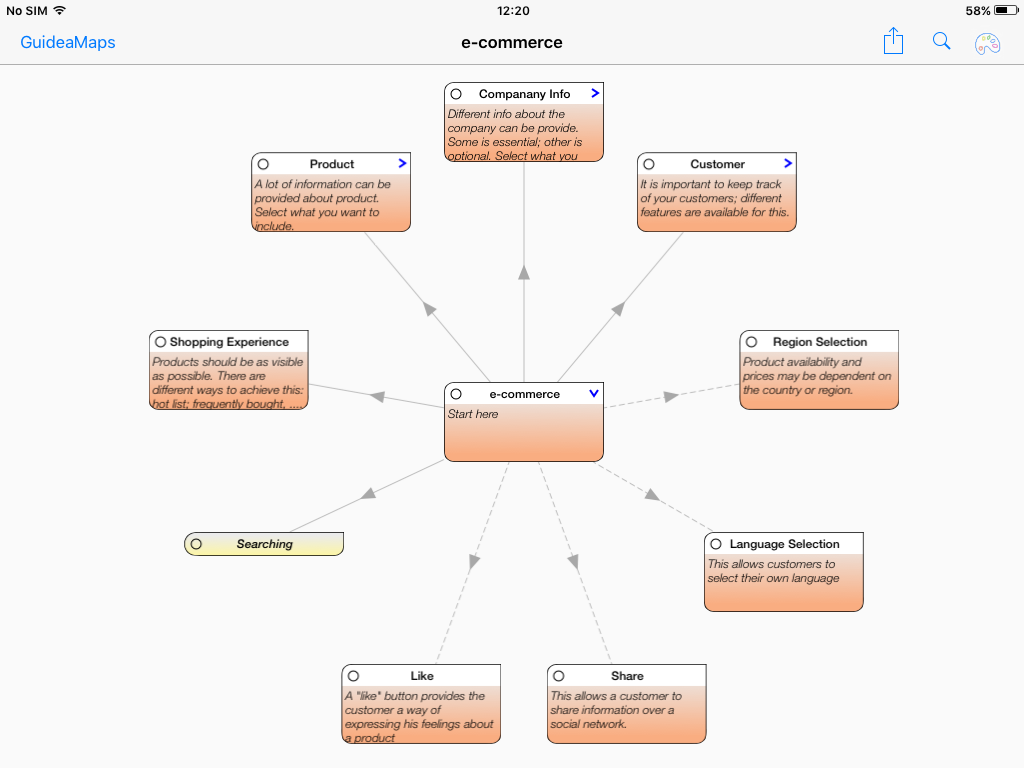
\includegraphics[width=\linewidth]{background/GMversion1ecommerce.png}}
	\caption{E-commerce example created in the original GuideaMaps application.}
	\label{fig:gm1.0-ecommerce}
\end{figure}


\clearpage

\chapter{Related Work}\label{ch:related-work}

There exist lots of ways to visualize data and the relations between data. In this chapter, we discuss visualization techniques related to the needs of GuideaMaps 2.0 (section \ref{sec:visualization-techniques}). In section \ref{sec:existing-tools}, we discuss related tools.


% ------------------------------------
% ----- VISUALIZATION TECHNIQUES -----
% ------------------------------------
\section{Visualization Techniques}\label{sec:visualization-techniques}

% ---------------------
% ----- MIND MAPS -----
% ---------------------
\subsection{Mind Maps}\label{sec:mind-maps}
The most well-known technique to visualize related data is to create a mind map (a.k.a. idea map). This technique is mainly used to show the relation between portions of information and for brainstorming purposes. Other applications where this technique is used are note-taking, and problem solving. \citep{knowledgemapsbalaid} \\

Mind maps are created by writing the main idea in the middle of the drawing, while all sub-ideas are placed around that center node. Each sub-idea is connected with its parent by means of a line. Hence, this kind of visualization is not difficult to create or understand. Its simplicity is one of the reasons why it is used a lot in practice.\\

Because mind maps is not a new concept, but one that most people already know quite well, we will only discuss one important aspect about this visualization technique. When using a digital version of mind maps, in general, the user can change the position of the nodes. \cite{wiegmann-1992} state that maps taking the Gestalt principles \citep{koffka2013principles} into account would be more performance-effective than maps that don't integrate Gestalt principles. Therefore, digital mind map systems usually allow their users to re-organize the nodes using drag and drop and by changing the color of the nodes. In this way, the user can, for example, put nodes containing similar data closer to each other and give them the same color (proximity and similarity principle).



% ----------------------------
% ----- VISUAL METAPHORS -----
% ----------------------------
\subsection{Visual Metaphors}\label{sec:visual-metaphors}
Another technique that can be used to represent content is the use of visual metaphors.

\begin{quote}
``A visual metaphor is a graphic structure that uses the shape and elements of a familiar natural or manmade artefact or of an easily recognizable activity or story to organize content meaningfully and use the associations with the metaphor to convey additional meaning about the content.'' \hfill \citep{eppler-2006}
\end{quote}

This technique could be used if you want to help users to memorize the most important elements of a topic, method or concept. In that case, you have to choose a metaphor which has properties in common with the topic, concept or method. \citep{eppler-2006} An example of a visual metaphor is shown in \autoref{fig:visual-metaphor}. It shows ``a mixed visual metaphor/conceptual diagram template to structure learning content in a narrative structure during a class room discussion'' \citep{eppler-2006}. 

\begin{figure}[H]
	\centering
	\frame{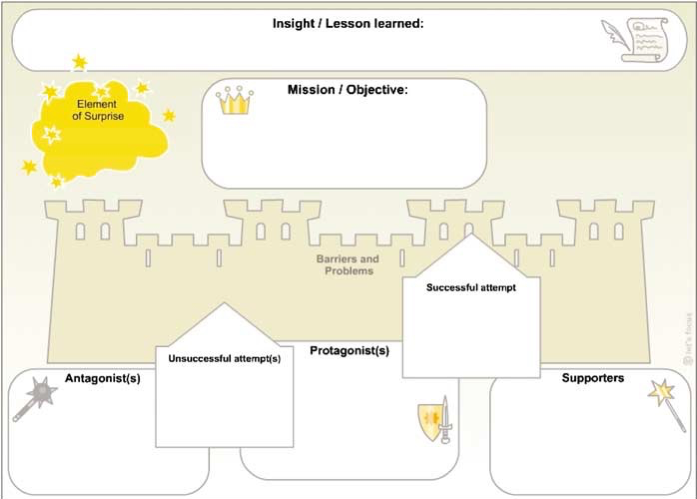
\includegraphics[width=0.75\linewidth]{visual-metaphor.png}}
	\caption{Example of a visual metaphor \citep{eppler-2006}.}
	\label{fig:visual-metaphor}
\end{figure}

As you can see in the figure, the visualization is completely adapted to the specific case of the topic. In this way, it is very difficult to create a generic metaphor, which can be used for different topics. As our tool should be usable for different topics, the technique of visual metaphors is less suitable for the needs of our tool.


% --------------------------
% ----- KNOWLEDGE MAPS -----
% --------------------------
\subsection{Knowledge Maps}\label{sec:knowledge-maps}
According to \cite{knowledgemapsbalaid}, \textit{knowledge maps} is an umbrella term for tools and techniques like mind maps. \cite{knowledgemapsodonnell} defined the concept as follows:

\begin{quote}
``Knowledge maps are node-link representations in which ideas are located in nodes and connected to other related ideas through a series of labeled links.'' \hfill 
\end{quote}

This way of representing information has for example a positive impact on students. The paper of \cite{knowledgemapsodonnell} teaches us that students using knowledge maps are better in remembering the main ideas of the subject in comparison to the ones that study from the text without the visualization. As GuideaMaps's purpose is more focused on representing large amounts of knowledge in an easy to grasp way, remembering the content is less important. However, the node-link representation with the main idea in the center also showed to be useful for this purpose, as illustrated by the popularity of mind maps.\\

Next to mind maps, concept maps is a second technique included under the umbrella of knowledge maps. Concept maps are in some sense similar to mind maps but they do have some different characteristics. First, the purpose of a mind map is to associate ideas, topics or things, while concept maps illustrate relations between concepts. Further, the structure of a concept map is mostly hierarchical and visualized like a tree. On the other hand, mind maps sometimes have a radial layout and not hierarchical. \citep{davies} \\

Hence, we can state that GuideaMaps makes use of a knowledge map visualization and more specifically some kind of combination of mind maps and concept maps.



% --------------------------
% ----- EXISTING TOOLS -----
% --------------------------
\section{Existing Tools}\label{sec:existing-tools}
In this section, we will discuss several already existing tools with similar functionality as defined in the goals of our application.

\subsection{Browser-based}
To create a digital mind map, a lot of browser-based tools exist yet. They are all very similar and only differ in a small number of functionalities. Therefore, we only discuss two examples of such tools.\\

Bubbl.us\footnote{\url{https://bubbl.us/}} is an online mind-mapping tool with very interesting features. Because it is browser-based, it works on all platforms and devices. Furthermore, you do not have to download any software to be able to use it. The biggest drawback of the system is that the nodes only contain a title. It is impossible to provide some content in addition to the title of the node. Hence, this tool is probably only useful to write down simple ideas instead of more complex structures of related data. Another drawback is that you can only change the color of the nodes but you can not customize their shape. But, as a user, you can drag and drop the nodes, share the visualization, work on it simultaneously, etc. Hence, Bubbl.us seems to be a well-created tool with lots of advantages. However, for the purpose of GuideaMaps 2.0, we need some functionality this tool does not provide.\\

A second browser-based tool is called ``MindMeister''\footnote{\url{https://www.mindmeister.com/}}. It is very easy to create an account, on which your different visualizations can be stored. Users are allowed to drag and drop the nodes to other positions and change their layout in terms of color and borders. However, you cannot show a preview of the content in the node itself. You always have to click the node to be able to see the content. Further, it is not possible to customize the links, which can be a drawback because now they are represented as a solid line and it is not possible to add an arrow on them. As a consequence, this is a second well-created tool with some important functionality missing.


\subsection{Moodle}

\cite{scherl2012moodle} described Moodle as follows:
\begin{quote}
	``Moodle is a widely used learning management system. It visualizes inner and interdisciplinary relations between learning objects and is generated dynamically depending on user set parameters and interactions. It is a free open-source software package that provides a course management system for the implementation of internet-based learning environments.''
\end{quote}

In Moodle, navigation between courses only works by binding URLs to words or pictures, like the way Wikipedia does it. This way of linking resources makes it difficult to  ``stay on top of things''. Therefore, \cite{scherl2012moodle} extended Moodle to provide a clear orientation throughout navigation. In this extended version, new learning activities can be linked to already existing learning activities in any course present in the Moodle platform. In so-called concept map-based navigation, the students can open a full-screen concept map (example in \autoref{fig:moodle-concept-map}). Every node represents a learning object and a click on it opens the corresponding resource. Further, currently visited learning object (node) is always in the center of the map, which is dynamically changed and updated based on user interactions. Hence, this system is comparable with the one we want to build: in our system, the currently selected node will be at the center as well and it should be possible to open nodes to see their content.

\begin{figure}[H]
	\centering
	\frame{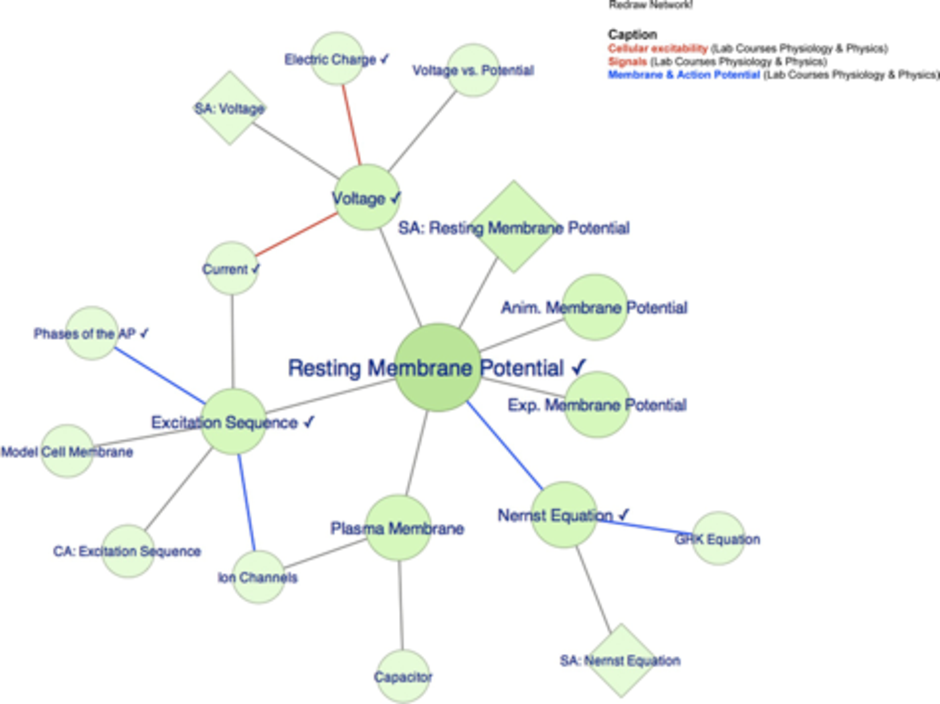
\includegraphics[width=0.75\linewidth]{relatedwork/moodle.pdf}}
	\caption{Example of concept map-based navigation in Moodle.}
	\label{fig:moodle-concept-map}
\end{figure}


\subsection{CmapTools}
In the paper of \cite{novak2006conceptmapping}, they did the following:
\begin{quote}
	``Extending the use of concept mapping to other applications such as the integration of concept mapping with the World Wide Web (WWW) led to the development of software that enhanced the potential of concept mapping, evolving into the current version of CmapTools now used worldwide in schools, universities, corporations, and governmental and non-governmental agencies. CmapTools is a client-server software tool to facilitate the construction and sharing of concept maps.''
\end{quote}

TODO: Another paper of cmaptools to discuss: \citep{canas2004conceptmapping}.\\







\clearpage

\chapter{User Classes \& Requirements}\label{ch:requirements}

In general, an application should meet a lot of requirements in order to deliver some quality to the users. A system should provide the right kind of functionality, but it should also be \textit{usable}, i.e. easy to learn and easy to use. Below are two definitions of usability which are often used:
\begin{description}
	\item[Definition 1] \hfill \\
	Usability is a measure of the ease with which a system can be learned and used, its safety, effectiveness and efficiency, and attitude of its users towards it. \hfill \citep{usability-definition-preece}

	\item[Definition 2] \hfill \\
	Usability is the extent to which a product can be used by specified users to achieve specified goals with effectiveness, efficiency and satisfaction in a specified context of use. \hfill \citep{usability-definition-improved}
\end{description}

Note that the second definition emphasizes the fact that usability is dependent on the target users and on the context of use. This means that one system can be usable for one type of user but not for another type of user or usable in one context but not in another context. Therefore, we also have to consider the different users of a system. In general, in user-centered design methods, the users are classified into user classes. Users in a user class are similar in terms of their characteristics and how they use the system.\\

Hence, we can distinguish between functional requirements and usability requirements. The system should meet the functional requirements to provide the right functionality and it should meet the usability requirements to be usable. There are also requirements that do not belong to either category, e.g. the so-called non-functional requirements.\\

This chapter starts by identifying the different user classes. Next, we will present and justify the major requirements formulated for our system, functional as well as usability requirements and other requirements. Detailed requirements and requirements that are rather straightforward are omitted here. Later in this thesis, when we explain the implementation details, we will come back to these requirements and discuss how we managed to meet them.



% ----------------------------------
% ---------- USER CLASSES ----------
% ----------------------------------
\section{User Classes}\label{sec:user-classes}
For our system, we can identify three user classes: (1) developer, (2) map creator and (3) end-user. The class the user belongs to will define its rights and possibilities. An overlap in the rights is possible, i.e. users of different classes can have a number of rights and possibilities in common. The different user classes are described into more detail in the following subsections.

\subsection{Developer}\label{sec:user-class-developer}
A developer is a user who can define and implement a custom visualization for the nodes and the links. This means that a developer can make sure that the tool can be used with a different visualization while the possibilities (in terms of functionality) are still the same. Developers are the only users that are able to do this because map creators and end-users are not allowed to extend the code with a custom implementation. The exact steps that need to be taken in order to provide a custom visualization in the tool are explained in chapter \ref{ch:implementation} and \ref{ch:usecase}.

\subsection{Map Creator}\label{sec:user-class-map-creator}
A map creator has the rights to create a so-called Guidea template or change the structure of an existing template. With the structure, we do not mean the layout of the nodes and the links, but the composition of the map itself. Hence, the map creator ``initializes'' the map by creating the nodes and links necessary for his goal. He provides a title and a description for each node. As a map creator, it is not possible to already provide the content of the node because that is the responsibility of the end-user. Note that this user corresponds to the template creator in GuideaMaps 1.0. However, in GuideaMaps 1.0 this had to be done in XML, while in our version it will be done in a graphical way \textcolor{blue}{to achieve \ref{goal:templates-graphical}}. We use the term ``map'' here (instead of template) because the term ``map'' is easier to understand than the term ``template'' by non-ICT schooled users.

\subsection{End User}\label{sec:user-class-end-user}
The end-user is the most restricted user in terms of rights and functionalities. He will use the map defined by a map creator and fill it with content. The end-user cannot change the title or the description, provided by the map creator, of a node but only provide the content. We have this restriction because otherwise this would give them the opportunity to change the structure of the map (which is a right reserved for the map creator). If the map creator did not provide this information, the end-user can add it, but never change it again afterwards, because, once the information is added, it is the same situation as when the map creator would have provided it.\\

\textcolor{blue}{
Further, an end-user is allowed to add child-nodes but they cannot delete nodes, because otherwise it would be possible for end-users to change the pre-defined map completely. The purpose of allowing the end-user to edit the map in some restricted way is to allow them to adjust the map to situations that were not foreseen by the map creator.
}


\color{blue}
% ----------------------------------
% ---------- REQUIREMENTS ----------
% ----------------------------------
\section{Requirements}\label{sec:requirements}

\subsection{Functional Requirements}\label{sec:functional-requirements}

% List of functional requirements
\begin{enumerate}[label=\textbf{FR \arabic*}., labelindent=0.5cm, ref=FR \arabic*, leftmargin=*]

	\item \label{fr:modes-rights}
		The system needs two modes: and end-user mode and a map creator mode. Depending on the mode used, the corresponding functionality should be available. 
	
	\item \label{fr:mapcreator:template}
		A map creator should be able to define a structure for the visualization and provide a title and description for each added node and options for choice nodes.
		
	\item \label{fr:customization} 
		\ref{goal:extend-modify} formulated earlier stated that the new version of GuideaMaps should allow the end-user to extend and modify the pre-defined map in some restricted way, i.e. they should be able to change the background color of nodes, to add missing child nodes, and it should also be possible to add new options in choice nodes. 
	
	\item \label{fr:delete-nodes}
		Map creators should be able to delete nodes as well, while end-users can only add missing ones.
		
	\item \label{fr:expand-collapse}
		Users should be able to collapse nodes to hide their children and expand nodes to show their children again.
  
	\item \label{fr:zoom}
		Zooming in or out such that you get less or more information at the same time on the screen is a frequently provided functionality for large visualizations. A feature to zoom is, for example, very useful in situations where you want to compare different parts of the visualization or focus on a certain part.
	
	\item \label{fr:zoom-to-fit}
		A variation on the zooming feature is ``zoom to fit'' (a.k.a. zoom until the complete figure fits into the bounding box). With custom zooming, the user can set the zooming level to meet its needs. Zoom to fit automatically adapts the zooming level and moves the content of the application until everything fits on the screen. This feature can, for example, be very useful to get an overview of the current data in the visualization.
		
	\item \label{fr:genericity}
		\ref{goal:generic} formulated earlier states that the application should be usable for different purposes. While GuideaMaps was usable in the context of domain specific requirement elicitation, our tool should also be useful in many other cases. Therefore, some requirements concerning the genericity of the application are needed:
  	\begin{enumerate}
		\item The tool should be generic in such a way that it is possible to use a different representation, e.g. shape/size for the nodes and the links.
		\item The default implementation should not be changed. An implementation for the nodes and the links created by a developer, should be \textit{plugged in} into the system, without affecting the default implementation.
	\end{enumerate}
	
	\item \label{fr:work-simultaneously}
		Multiple users should be able to work on the same visualization at the same time.
  
\end{enumerate}



\subsection{Usability Requirements}\label{sec:usability-requirements}

% List of usability requirements
\begin{enumerate}[label=\textbf{UR \arabic*}., ref=UR \arabic*, labelindent=0.5cm, leftmargin=*]

	\item \label{ur:intuitiveness}
		The tool should not only be used by people with experience in Computer Science. It does not matter whether or not the user has a background in Computer Science, he should be able to easily learn to use the system in a short time.
	
	\item \label{ur:icons}
		Possible actions should be labeled by clear, not misunderstandable icons. The icons should not be ambiguous, they should link to one particular action and thus the user should know exactly what to expect when clicking on the icon. Well chosen icons are one of the factors in the design that contribute to learnability and ease of use.
	
	\item \label{ur:gestures}
		Gestures for common actions should not differ from the gestures used for the same action in other applications. (e.g. the scrolling gesture is probably the best gesture for zooming, because this is a well-known way to zoom in applications (e.g. Google Maps). Using the same gesture as in other applications will improve the learnability of our tool.)
	
	\item \label{ur:accessibility}
		The target audience of the application should be limited as little as possible: color blind people should still be able to use the system.
	
	\item \label{ur:time}
		To save time, end-users should be able to add extra options to choice nodes without having to contact the map creator to update the options.
	
\end{enumerate}



\subsection{Other Requirements}\label{sec:other-requirements}

\begin{enumerate}[label=\textbf{OR \arabic*}., ref=OR \arabic*, labelindent=0.5cm, leftmargin=*]
	\item \label{or:device-os-independent}
		To achieve \ref{goal:device-os-independent}, the application should run on different kinds of devices (e.g. tablets, laptops and desktops) and operating systems (Android, iOS, MacOS and Windows). While version 1.0 was only designed for an iPad, our version should provide a solution for this restriction.\\
	
	The only restriction on the used device is that it needs to have a screen that is large enough because it is not very convenient to work with the visualization on small screen areas, e.g. on smartphones. The application could run on smartphones but it is not recommended nor required to use it on devices with relatively small screens.
	
	\item \label{item:code-separation}
		The core of the application should be completely separated from custom implementations created by developers.

\end{enumerate}

\color{black}

\clearpage

\chapter{Implementation}\label{ch:implementation}

The previous sections explained \textit{what} the application should do, which goals should be achieved and which requirements we surely want the application to meet. In this section, more details are provided about \textit{how} all this is translated to an implementation.

\section{Web Application}
Before we started with the actual implementation, we had to decide how to achieve \ref{goal:device-os-independent}, i.e. how will we make sure the application is device- and OS-independent? (Requirement section \ref{sec:other-requirements}) A first technique could have been to make use of the Java Virtual Machine. This approach would work but we want to make it possible to let multiple people work on the same visualization (\ref{fr:work-simultaneously}), eventually at the same time. Therefore, it is more convenient to have a browser-based application, i.e. Web Application.\\

Nowadays, a lot of browsers exist, each with their own characteristics and differences. Because the goal of this thesis was to have a functional prototype, it is not required that the application works perfectly on \textit{all} possible browsers. However, we wanted to make sure that the tool works without any issues in one of the most popular browsers, being Google Chrome.\\

\textcolor{blue}{
Another possibility would have been to use cross-platform tools like PhoneGap\footnote{\url{https://phonegap.com/}} and Cordova\footnote{\url{https://cordova.apache.org/}}. The benefit of those tools is that, if a real application is preferable to a browser-based application, it is still possible to wrap the browser app into a real app. Hence, from then on the application can be installed on the device itself. A drawback of this is that the app cannot be used if the device has not enough disk space. Further, the app is possibly not up-to-date at any time. This can become an issue when the app would be collaborative and multiple users with different versions of the app want to work with it. Therefore, we concluded that a browser-based solution is better for our goal than the Java Virtual Machine and cross-platform tools.
}

% --------------------
% --- TECHNOLOGIES ---
% --------------------
\section{Used Technologies}\label{sec:technologies}
A lot of technologies exist to create Web applications and visualizations. A number of technologies assist in the developing process of such an application. In the following subsections we present the selected technologies, as well as why we chose for this particular technology and not for the alternatives.

\subsection{ReactJS}\label{sec:reactjs}
ReactJS\footnote{\url{https://reactjs.org/index.html}} is an open source library to create user interfaces. One of its main goals is to provide the best possible rendering performances\footnote{\url{https://medium.com/@thinkwik/why-reactjs-is-gaining-so-much-popularity-these-days-c3aa686ec0b3}}. Performance is good because ReactJS allows developers to break down the user interface into different components. Each component has its own \textit{state}, which contains information about the content of the component. This state can be updated while the application is running and if such an update is made, only this component is re-rendered instead of re-rendering the complete UI\footnote{\url{https://facebook.github.io/react/docs/why-react.html}}. Hence, this provides a huge benefit for the performance. Next to that, it is also not very hard to learn to code in React comparing to other frameworks (e.g. AngularJS). If the developer knows HTML and JavaScript, he will be able to code in ReactJS quickly.\\

Because of these benefits, ReactJS is the framework in which the GuideaMaps application is implemented. Each node and each link is considered as a separate and unique React Component. The most important reason for implementing the nodes like this is performance: if the state of the node is updated, only this node is re-rendered and not the complete UI.\\

Alternatives for ReactJS are for example AngularJS and VueJS\footnote{https://medium.com/@TechMagic/reactjs-vs-angular5-vs-vue-js-what-to-choose-in-2018-b91e028fa91d}. ReactJS is by far the most used of these three. Further, it is said to be easier to learn because you only have one structure (``Component''), while in AngularJS this is not the case. Also, VueJS lacks resources and is not used a lot in practice, which makes it more difficult to discuss problems with other developers. Maybe the most important benefit of ReactJS is its performance; React is really fast and our tool should have fast rendering times as well. Hence, because the alternatives seem to have some important drawbacks, we chose for ReactJS as the framework for creating the application. 

\subsection{d3}\label{sec:d3}
Another helpful tool is d3. With d3-hierarchy\footnote{\url{https://github.com/d3/d3-hierarchy}}, it is possible to transform JSON-data into hierarchical data. Having this kind of data makes it much easier to create a tree- or cluster-structure. In the case of GuideaMaps, a clustered visualization is very useful. The \textit{main}-node (a.k.a. the root node) is then positioned at the center, such that its child nodes can be placed around it. Hence, the further a node is away from the center, the lower it is in the hierarchy. Also, the visualization will not be messed up by positioning the nodes in this way, because every node has exactly one parent. This means there will not be a spaghetti of links where you cannot see from which node the link comes and to which node it is pointing.\\

Further, d3 makes it easier to create a zoomable layout. The tool is able to update the positions of the nodes each time the zooming level is changed. Hence, as a developer, you do not have to take care of the updated positions if you make use of d3. By using this technique, the functional requirements about zooming (\ref{fr:zoom} and \ref{fr:zoom-to-fit}) are easily achieved.\\

The alternatives for d3 most of the time come with a problem d3 does not have. For example ChartJS and ChartistJS are limited in the number of features: you can create nice charts with it, but d3 provides more visualizations than only charts. Further, some of the alternatives are commercial (Highcharts, Webix). d3 is open-source and provides functionality to zoom, to create a cluster of nodes based on JSON-data describing these nodes, etc. Because of the wide range of possibilities with d3, the fact that it is widely used and supported by all modern browsers and that it is able to act together with ReactJS, we believe that d3 was a better choice than its alternatives. 

\subsection{Tailwind CSS}\label{sec:tailwind}
Nowadays, the ``look and feel'' of an application is very important. Everything should look pretty and, as already mentioned in section \ref{sec:usability-requirements}, the actions should be straightforward and visible. Implementing a nice style can require a lot of code. The code for these styles can become a big part of the implementation. Hence, a good framework is necessary to reduce the lines of style code to a reasonable number and to help to improve the readability of the code.\\

Tailwind CSS\footnote{\url{https://tailwindcss.com/}} is a framework that assists developers to style their application. The difference with more famous frameworks, like Bootstrap, is that Tailwind CSS has no default theme. If you want to use a Bootstrap-feature, this eventually comes along with other features you do not always want and it can be quite hard to undo the part you do not want. Furthermore, you have to write additional lines of style code to undo the unwanted parts. With tailwind on the other hand, you can grab only the features you want, without side-effects. \autoref{fig:examplecode-tailwindcss} shows an example with two small listings. The first uses inline style while the second makes use of tailwind CSS.

\begin{figure}[H]
	\begin{minipage}[b]{0.5\textwidth}
 		\centering
  		\begin{minted}[linenos, escapeinside=||]{html}
<div
  style={{
    |\textcolor{red}{position:}| absolute|,|
    |\textcolor{red}{border:}| 1px solid black|,|
    |\textcolor{red}{borderRadius:}| O.25rem|,|
    |\textcolor{red}{padding:}| 0.5rem|,|
  |\textcolor{red}{\}\}}|
/>
		\end{minted}
		\label{lst:no-tailwind}
		\captionof{lstlisting}{Normal CSS, no tailwind.}
	\end{minipage}
 	\begin{minipage}[b]{0.5\textwidth}
  		\centering
		\begin{minted}[breaklines, escapeinside=||]{html}
<div
  className={
    |'|absolute border border-solid border-black rounded p-2|'|
  |\textcolor{red}{\}}|
/>
		\end{minted}
		\label{lst:tailwind}
 	 	\captionof{lstlisting}{With tailwind CSS.}
 	\end{minipage}
	\caption{Difference when using tailwind CSS or not.}
	\label{fig:examplecode-tailwindcss}
\end{figure}

The figure illustrates the difference to implement four CSS property-value pairs in normal CSS and implementing the same four with tailwind. In the case of normal CSS, we need four lines of code to obtain the intended result. On the other hand, with tailwind CSS, we add some classes providing the same style. By using these classnames, the developer can see the properties faster than with normal CSS. Hence, in case of lots of lines of CSS code, tailwind can be faster to use compared to normal CSS.\\

Bootstrap can be very interesting to use in applications and websites that should run on devices with small screens (e.g. smartphones). But we decided not to tailor our application for such devices (section \ref{sec:other-requirements}). Given the example and the fact that Tailwind CSS does not have a default theme, we prefer Tailwind over Bootstrap. Keep in mind that it is certainly possible to create the same application with Bootstrap, but with Tailwind CSS, the code will be easier to understand.\\





% ---------------------
% ----- STRUCTURE -----
% ---------------------
\section{Main Code Structure}\label{sec:structure}
With the technologies mentioned in the previous section, the most important pillars the application relies on are discussed. In this section, we will explain the main structure of the code, such that it is clear how all elements work together. Figure \ref{fig:overall-structure} shows a visualization of the structure of the code.
\begin{figure}[H]
	\centering
	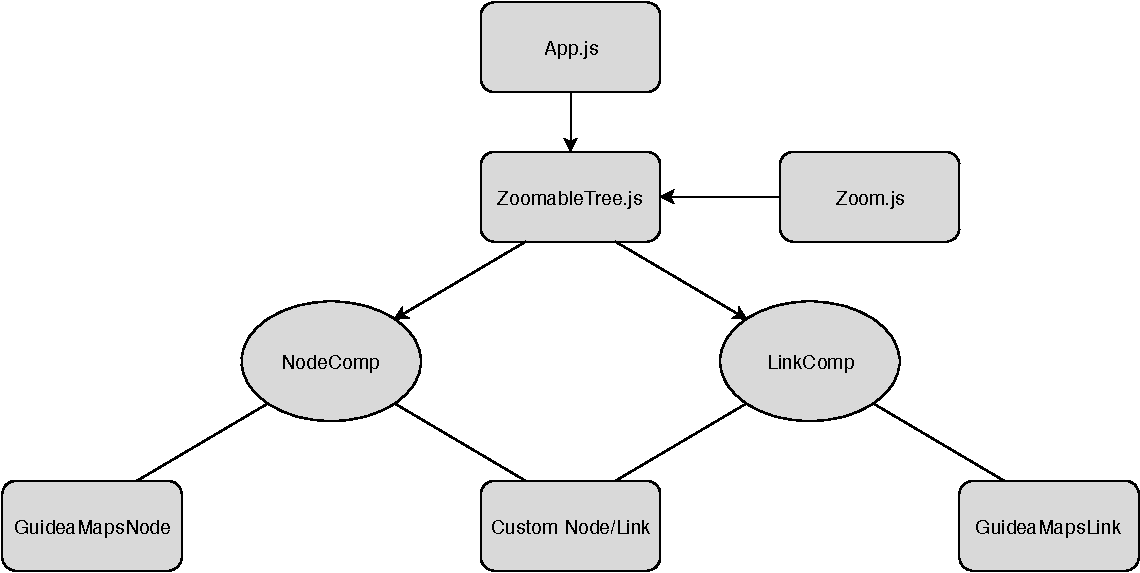
\includegraphics[width=\linewidth]{thesis-architecture.pdf}
	\caption{Structure of the application.}
	\label{fig:overall-structure}
\end{figure}

The application is developed in such a way that it can be used as a library for other purposes than GuideaMaps. In this way, \ref{goal:generic} to have a generic solution will be achieved. The general, always-returning part of the code can be found in App.js, ZoomableTree.js and Zoom.js, where the layout of the nodes is defined as well as the implementation to allow the user to zoom the visualization in and out. To realize the library, the layer of the NodeComp and LinkComp is very important. For GuideaMaps (shorthand GM), an implementation for NodeComp and LinkComp, being GMNode and GMLink is provided. Each implementation describes how every node and every link should look like in the visualization. When a particular user would like to have a different representation for the nodes or the links or both, new components (e.g. MyCustomNode and MyCustomLink) should be implemented. In the rest of the code, only one line should be adapted: in App.js, ZoomableTree is called with a certain number of props. Two of these props are NodeComp and LinkComp, which are set to GMNode and GMLink, respectively, by default. Hence, the only action that is required to \textit{plug in} an other component is replacing GMNode and GMLink by this component (e.g. MyCustomNode and/or MyCustomLink). Hence, the visualization can be customized to the needs of the user and \ref{fr:customization} is achieved. \autoref{fig:examplecode-library} shows the part of the code in App.js that should be adapted as explained. Note that the shown props are not the only props that are passed to ZoomableTree. The others are omitted for readability.\\

The reason why we chose for this approach is that now the developer does not have to change anything of the default implementation. He only has to create his own components and plug them in as props for ZoomableTree and leave the rest of the implementation as it is.\\

\begin{figure}[H]
	\begin{minipage}{0.5\textwidth}
 		 \centering
		 \begin{minted}[linenos, escapeinside=||]{html}
<ZoomableTree
    |\textcolor{mygreen}{NodeComp}|=|\textcolor{red}{\{GMNode\}}|
    |\textcolor{mygreen}{LinkComp}|=|\textcolor{red}{\{GMLink\}}|
/>
		\end{minted}
		\label{lst:default-components}
		\captionof{lstlisting}{Default components.}
	\end{minipage}
 	\begin{minipage}{0.5\textwidth}
  		\centering
  		\begin{minted}[escapeinside=||]{html}
<ZoomableTree
    |\textcolor{mygreen}{NodeComp}|=|\textcolor{red}{\{MyCustomNode\}}|
    |\textcolor{mygreen}{LinkComp}|=|\textcolor{red}{\{MyCustomLink\}}|
/>
		\end{minted}
		\label{lst:custom-components}
 	 	\captionof{lstlisting}{Custom components.}
 	\end{minipage}
	\caption{Two listings showing how to use the library.}
	\label{fig:examplecode-library}
 	%\captionof{figure}{Two listings showing the difference between the default and custom use of the library.}
\end{figure}

Next to custom components, a developer can also implement his own functions to handle changes in the visualization. For example, to add a new child node, GuideaMaps calls the function passed to the \textit{onAddNode}-prop (i.e. addGMChildNode). In a custom implementation, you can pass another function to this prop to make sure that other work is done. If you do not want to allow users to add child nodes, you do not have to remove this line but you just replace addGMChildNode by \textit{() -> null}, a function that does not do anything (because the library is created in a way to avoid changes in the default code structure). It is not wrong to keep addGMChildNode as parameter, but if the function would be called, this can lead to errors or wrong behaviour of the application. Therefore, we recommend to always pass \textit{() -> null} as argument to functions that should not be used. More details about the use of the library can be found in Chapter \ref{ch:usecase}, where a complete use case is elaborated.



% ------------------------------
% ----- GUIDEAMAPS DETAILS -----
% ------------------------------
\section{Default Implementation: GuideaMaps}
Now the overview of the structure of the application has been discussed, we will consider the GuideaMaps visualization and its implementation details in this section. An example visualization can be seen in \autoref{fig:guideamaps}.\\

The nodes represent a specific part of the data and the links illustrate the relation between the data (i.e. the nodes). Before we discuss the nodes into detail, we start with the \textit{navigation bar} above the visualization itself. This navigation bar is divided in three equal parts. In the center, the user can select via an option menu which map or template he wants to use. The name of the selected option is always visible. This functionality is available because the user should be able to switch between different tasks. In each task, the user can work with a different map or start a new map based on one of the existing templates, created by a map creator.\\

The right part of the navigation bar contains a single button. A click on this button makes sure the visualization is zoomed in such a way that all nodes fit in the window. This is one of the reasons why we mentioned in the requirements (section \ref{sec:other-requirements}) that the screen of the used device should not be too small. If the screen is too small, the nodes of a larger visualization will overlap each other because otherwise they would not fit all on the screen. When nodes overlap, a lot of information can be hidden and the visualization can become useless.

\begin{figure}[h]
	\centering
	\frame{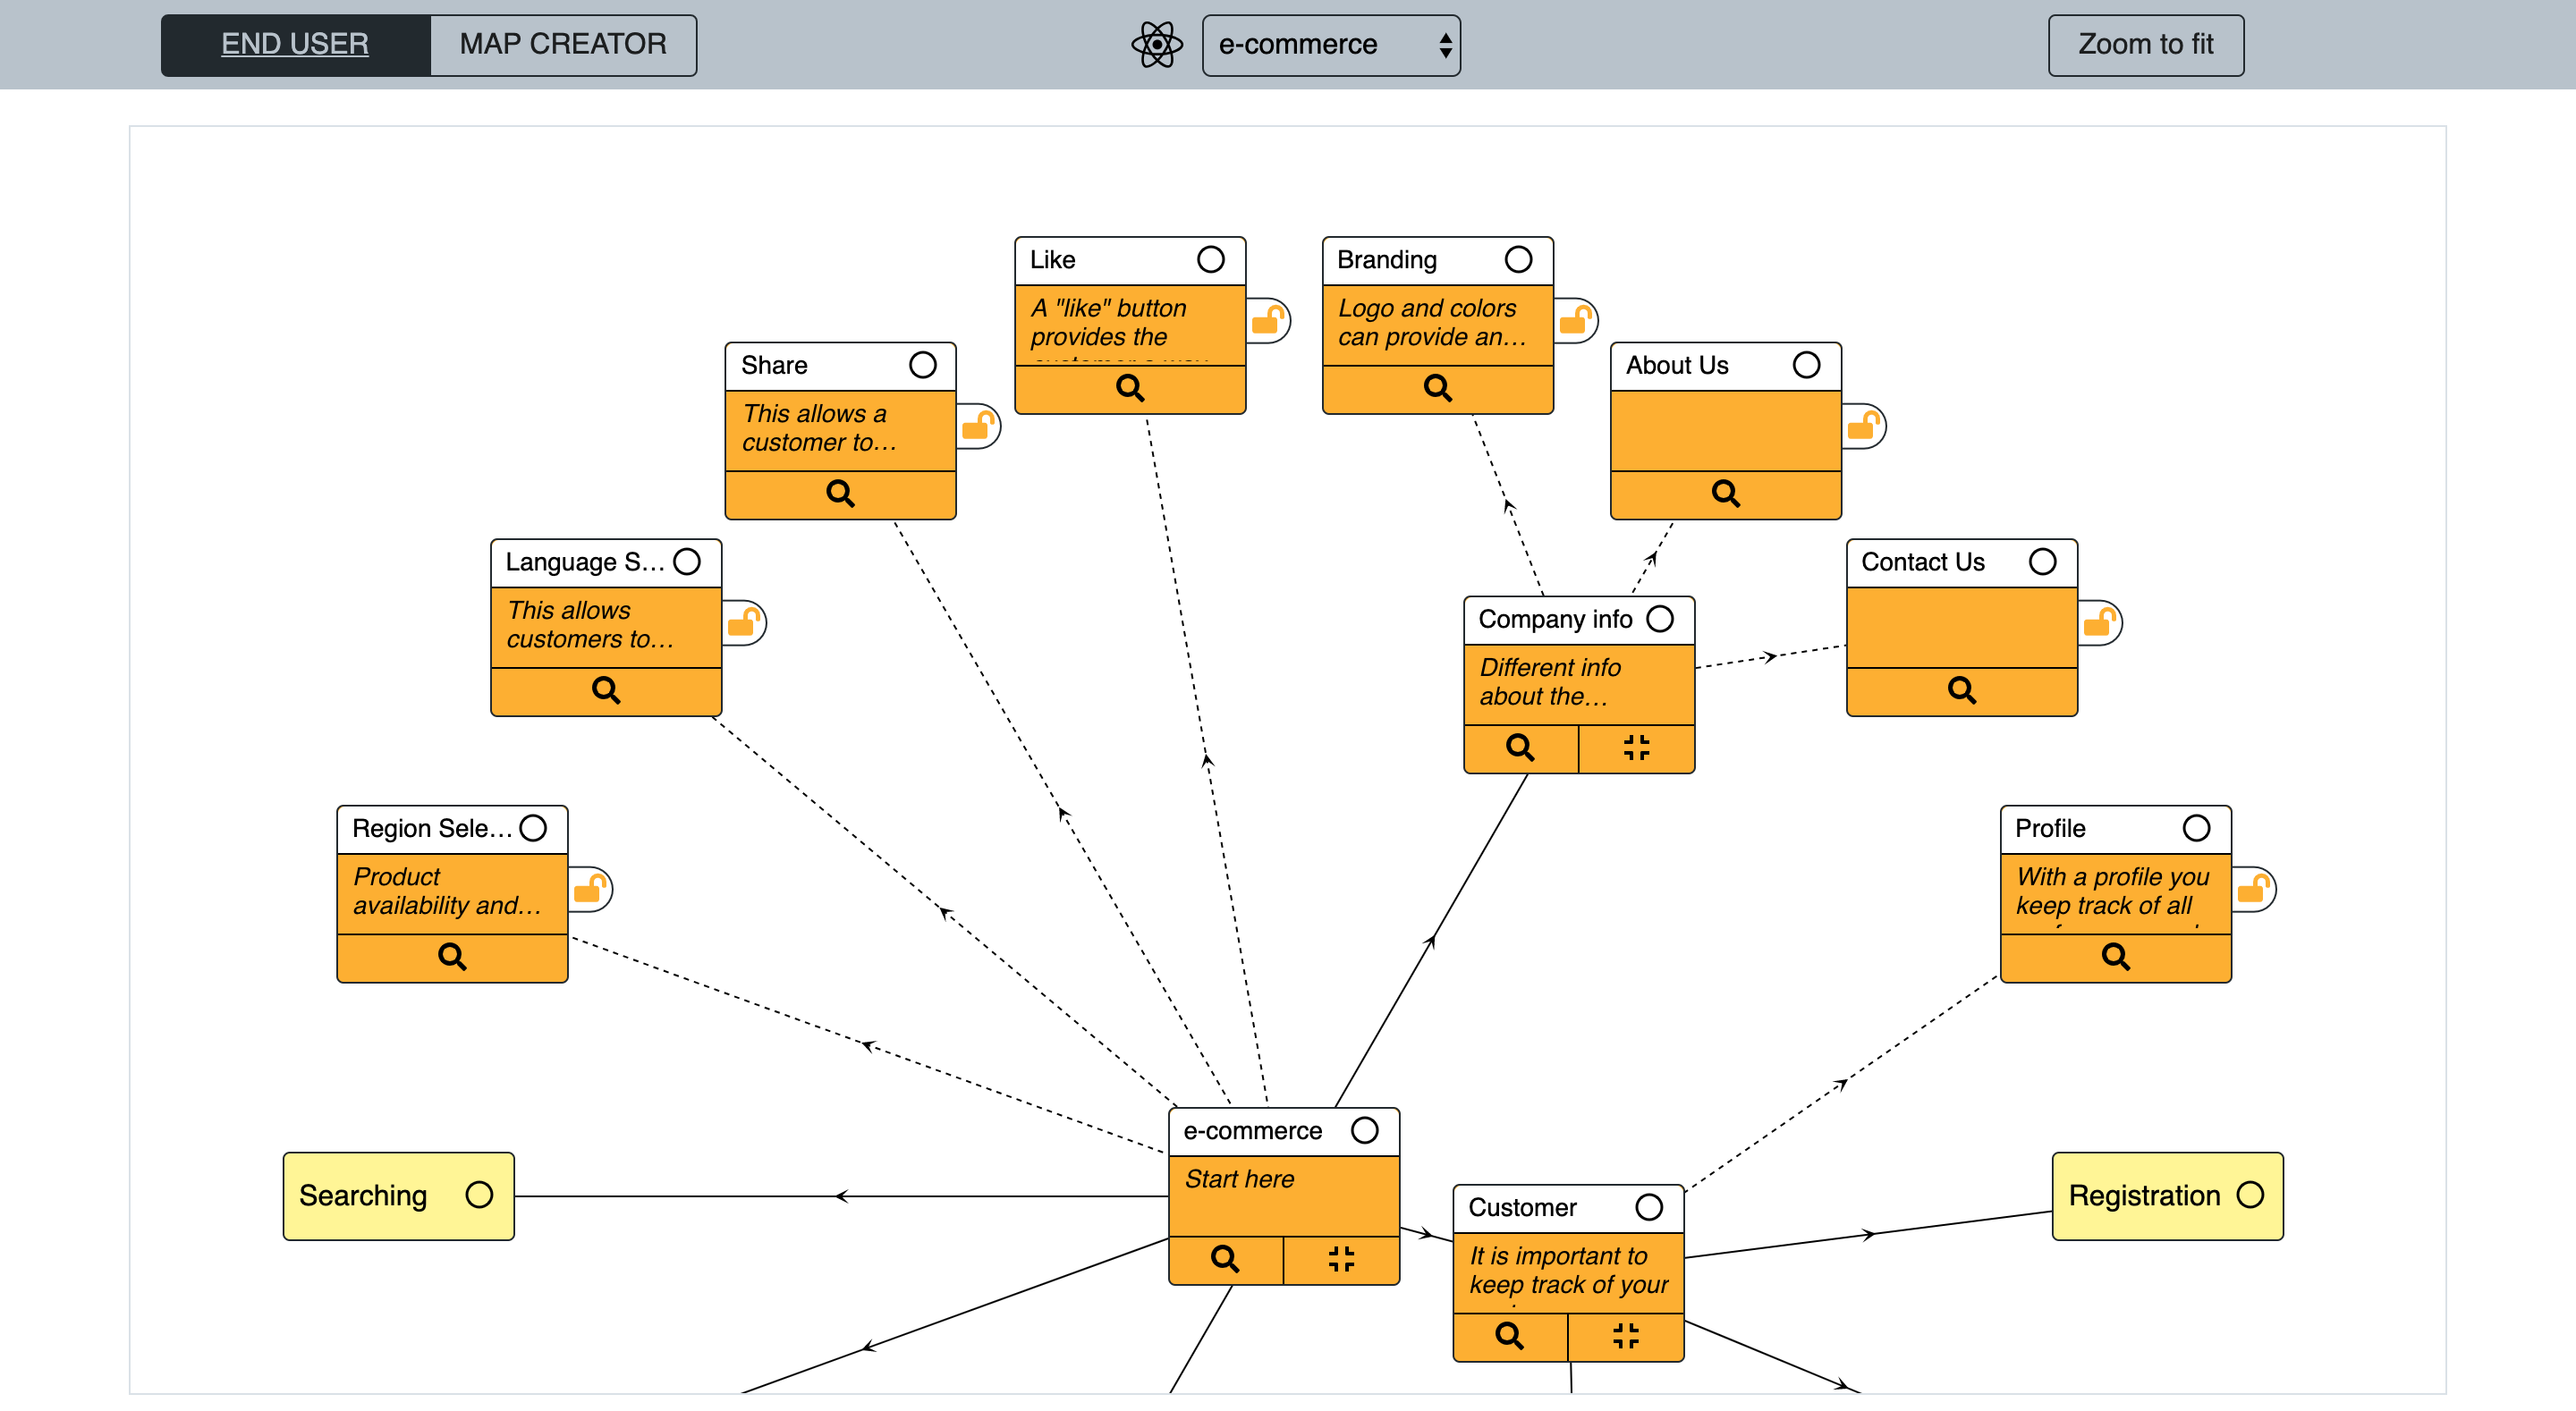
\includegraphics[width=\linewidth]{guideamaps.png}}
	\caption{GuideaMaps Layout.}
	\label{fig:guideamaps}
\end{figure}

The left part of the navigation bar is created to be able to switch between the user modes (i.e. end user or map creator). As required, a map creator has more rights and hence he can perform more actions than an end-user. In the following subsections, the differences between these modes are elaborated.





% ---------------------------
% ------ REGULAR NODES ------
% ---------------------------
\subsection{Regular Nodes}

\begin{figure}[H]
	\centering
	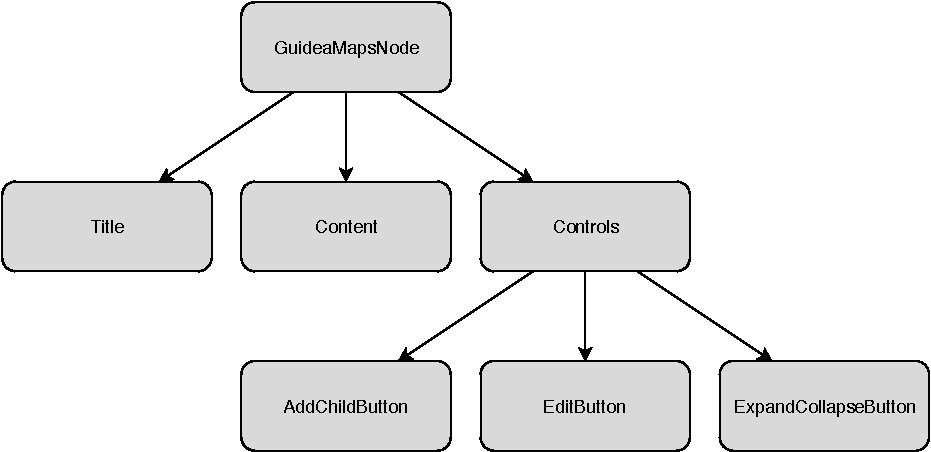
\includegraphics[width=\linewidth]{GMStructure.pdf}
	\caption{Structure of GuideaMapsNode.}
	\label{fig:gmnodestructure}
\end{figure}

As you can see in \autoref{fig:gmnodestructure}, the structure of a GuideaMapsNode node is quite simple. Each node consists of three html \textit{div}-elements: a title-div, a content-div and a controls-div explained below.

\addtocontents{toc}{\protect\setcounter{tocdepth}{2}} % hide the following subsections from the table of contents
\subsubsection{Title}
The title-div is positioned at the top of the node. It consists of the title text when this is given by the map creator. Otherwise, it shows \textit{Insert title} in italics to remind the user that he still has to set a title for this node. An end-user can set the title if no title exists yet, but he can never change it. The reason for this is because we distinguish two situations. In the first situation, the end-user adds a child node for a particular parent. This node has no title by default and then he should be able to insert a title. In the second situation, the user opens an existing node created by the map creator. In that case the end-user is not allowed to change the title of the node, because otherwise he would be able to change the meaning of the node. \\

Next to the title-text, the title-div contains an icon placed near the right border. This icon indicates to an end-user whether all information for the node, i.e. content, is provided or not. The icon that is shown also depends on whether the information in the child-nodes is given or not. We distinguish three possible situations:
\begin{enumerate}
	\item The node itself and all of its (non-optional) children are correctly filled in. In this case the icon will be a completely filled circle.
	\item The node itself and all of its (non-optional) children are still empty. In this case the icon will be an empty circle.
	\item In all other cases, the node itself or at least one of its child-nodes is filled. Then the icon will be a semi-filled circle.
\end{enumerate}
This icon can assist the end-user in determining whether all information requested by a template is given. For example, if he checks the root node and sees that the circle is completely filled, he knows that all mandatory information in every child-node is given. On the other hand, suppose only one node does not yet contain the required content, then the user starts from the root node and always follows the child-node with a semi-filled circle. In this way, he will find the incomplete node much faster than in the case he has to check all the nodes, one by one. Hence, the icon is an element that helps to improve the usability of the application.



\subsubsection{Content}\label{sec:content}
The content of each node is some text describing the information required for the node. As long as no content is provided by the end-user, the description provided by the map creator is shown in italics to instruct the end-user which content to provide.



\subsubsection{Controls}\label{sec:controls}
The last part of a node is the controls-div. With \textit{controls} we mean the different actions a user can take concerning the particular node. As actions, a user can (a) add child nodes, (b) explore and edit data of a node, (c) expand and (d) collapse a node. As mentioned in the Usability Requirements (section \ref{sec:usability-requirements}), it is very important to choose for non-misunderstandable icons. Therefore, we chose for the following icons (\autoref{fig:icons}).

\begin{figure}[H]
	\centering
	\begin{subfigure}{.2\textwidth}
  		\centering
  		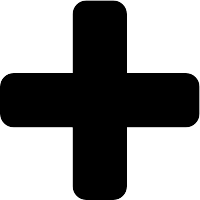
\includegraphics[width=.25\linewidth]{plusicon}
  		\caption{Plus}
  		\label{fig:plusicon}
	\end{subfigure}%
	\begin{subfigure}{.2\textwidth}
  		\centering
  		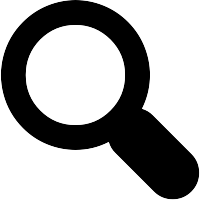
\includegraphics[width=.25\linewidth]{magnifyingicon}
  		\caption{Explore/Edit}
  		\label{fig:editicon}
	\end{subfigure}
	\begin{subfigure}{.2\textwidth}
		\centering
  		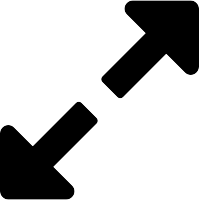
\includegraphics[width=.25\linewidth]{expandicon}
  		\caption{Expand}
  		\label{fig:expandicon}
	\end{subfigure}
	\begin{subfigure}{.2\textwidth}
  		\centering
  		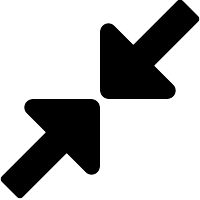
\includegraphics[width=.25\linewidth]{collapseicon}
  		\caption{Collapse}
  		\label{fig:collapseicon}
	\end{subfigure}
	\caption{Good icons for the following actions: (a) add child node, (b) explore and edit node, (c) expand node and (d) collapse node.}
	\label{fig:icons}
\end{figure}

The number of actions a user can perform depends on the mode. An end-user has two buttons: one to ``open'' the node to view and edit the data, and one to expand or collapse the node, i.e. to show or hide the child nodes, respectively. When a node is collapsed, all child nodes on all lower levels in the hierarchy are hidden. On the other hand, when a node is expanded, only the child-nodes of the next level in the hierarchy are shown.\\

Because a map creator is allowed to add child nodes, a third button can be found in his controls-div of the node to add a child node. A click on this button opens a small modal window, where some information about the new node should be provided before the node can be created. \autoref{fig:gm-add-general} illustrates what the modal window looks like when the user wants to add a regular node. He has to start by selecting the option ``Default'' at the top, after which two input fields appear to insert the title and the description for the node. A click on the button at the bottom will add a child node of the selected type and with the provided title and description.\\

It is possible to add an \textit{empty} node if the user does not provide a title and/or a description. Even though it is not really useful to add nodes without any context, we only require the user to select the type of the child node. If the type is unknown, the node will not be added. A situation where a map creator would add an empty node is when he wants to remind himself that a child node is necessary at that place, but details about the expected content are not yet known.\\

\begin{figure}[H]
	\centering
	\frame{\includegraphics[width=\linewidth]{GMAddChildNodeModal-General.png}}
	\caption{Adding a general node.}
	\label{fig:gm-add-general}
\end{figure}



\subsubsection{EditModal Window}\label{sec:editmodal}
A click on the button to open the node opens a modal window containing the data. What this modal window looks like depends on the mode. If we are in map creator mode, a form will be shown to allow to change the title, the description, and the background color (see \autoref{fig:gm-editmodal-mapcreator}). In the case of the end-user mode (see \autoref{fig:gm-editmodal-enduser}), only the content and the background color can be changed. Only the first time a child node is added and no title and description is available yet, the end user is able to fill in these data as well.\\

When changing the background color, the user can choose to use the color also for all children or not. If the checkbox ``include children'' is checked, the background color of all child-nodes on all sublevels in the hierarchy will be changed to the new color. Otherwise, only the background color of the current node will be changed.\\

The text color is black by default. This can become a problem when the background color is changed to a dark color and certainly when it is black as well because then the text is not readable anymore. To solve this issue, we wrote some CSS rules that change the text-color depending on the background color. A black (or dark) background will result in white text and a white (or light) background results in black text.\\

The possibility to change the background color of the nodes and the fact that the text color is adapted taking the background color into account is also a useful feature for color-blind people. In this way, they can adapt the background colors of the nodes to colors they can distinguish better. Hence, requirement \ref{ur:accessibility} is achieved by this functionality.

\begin{figure}[H]
	\centering
	\frame{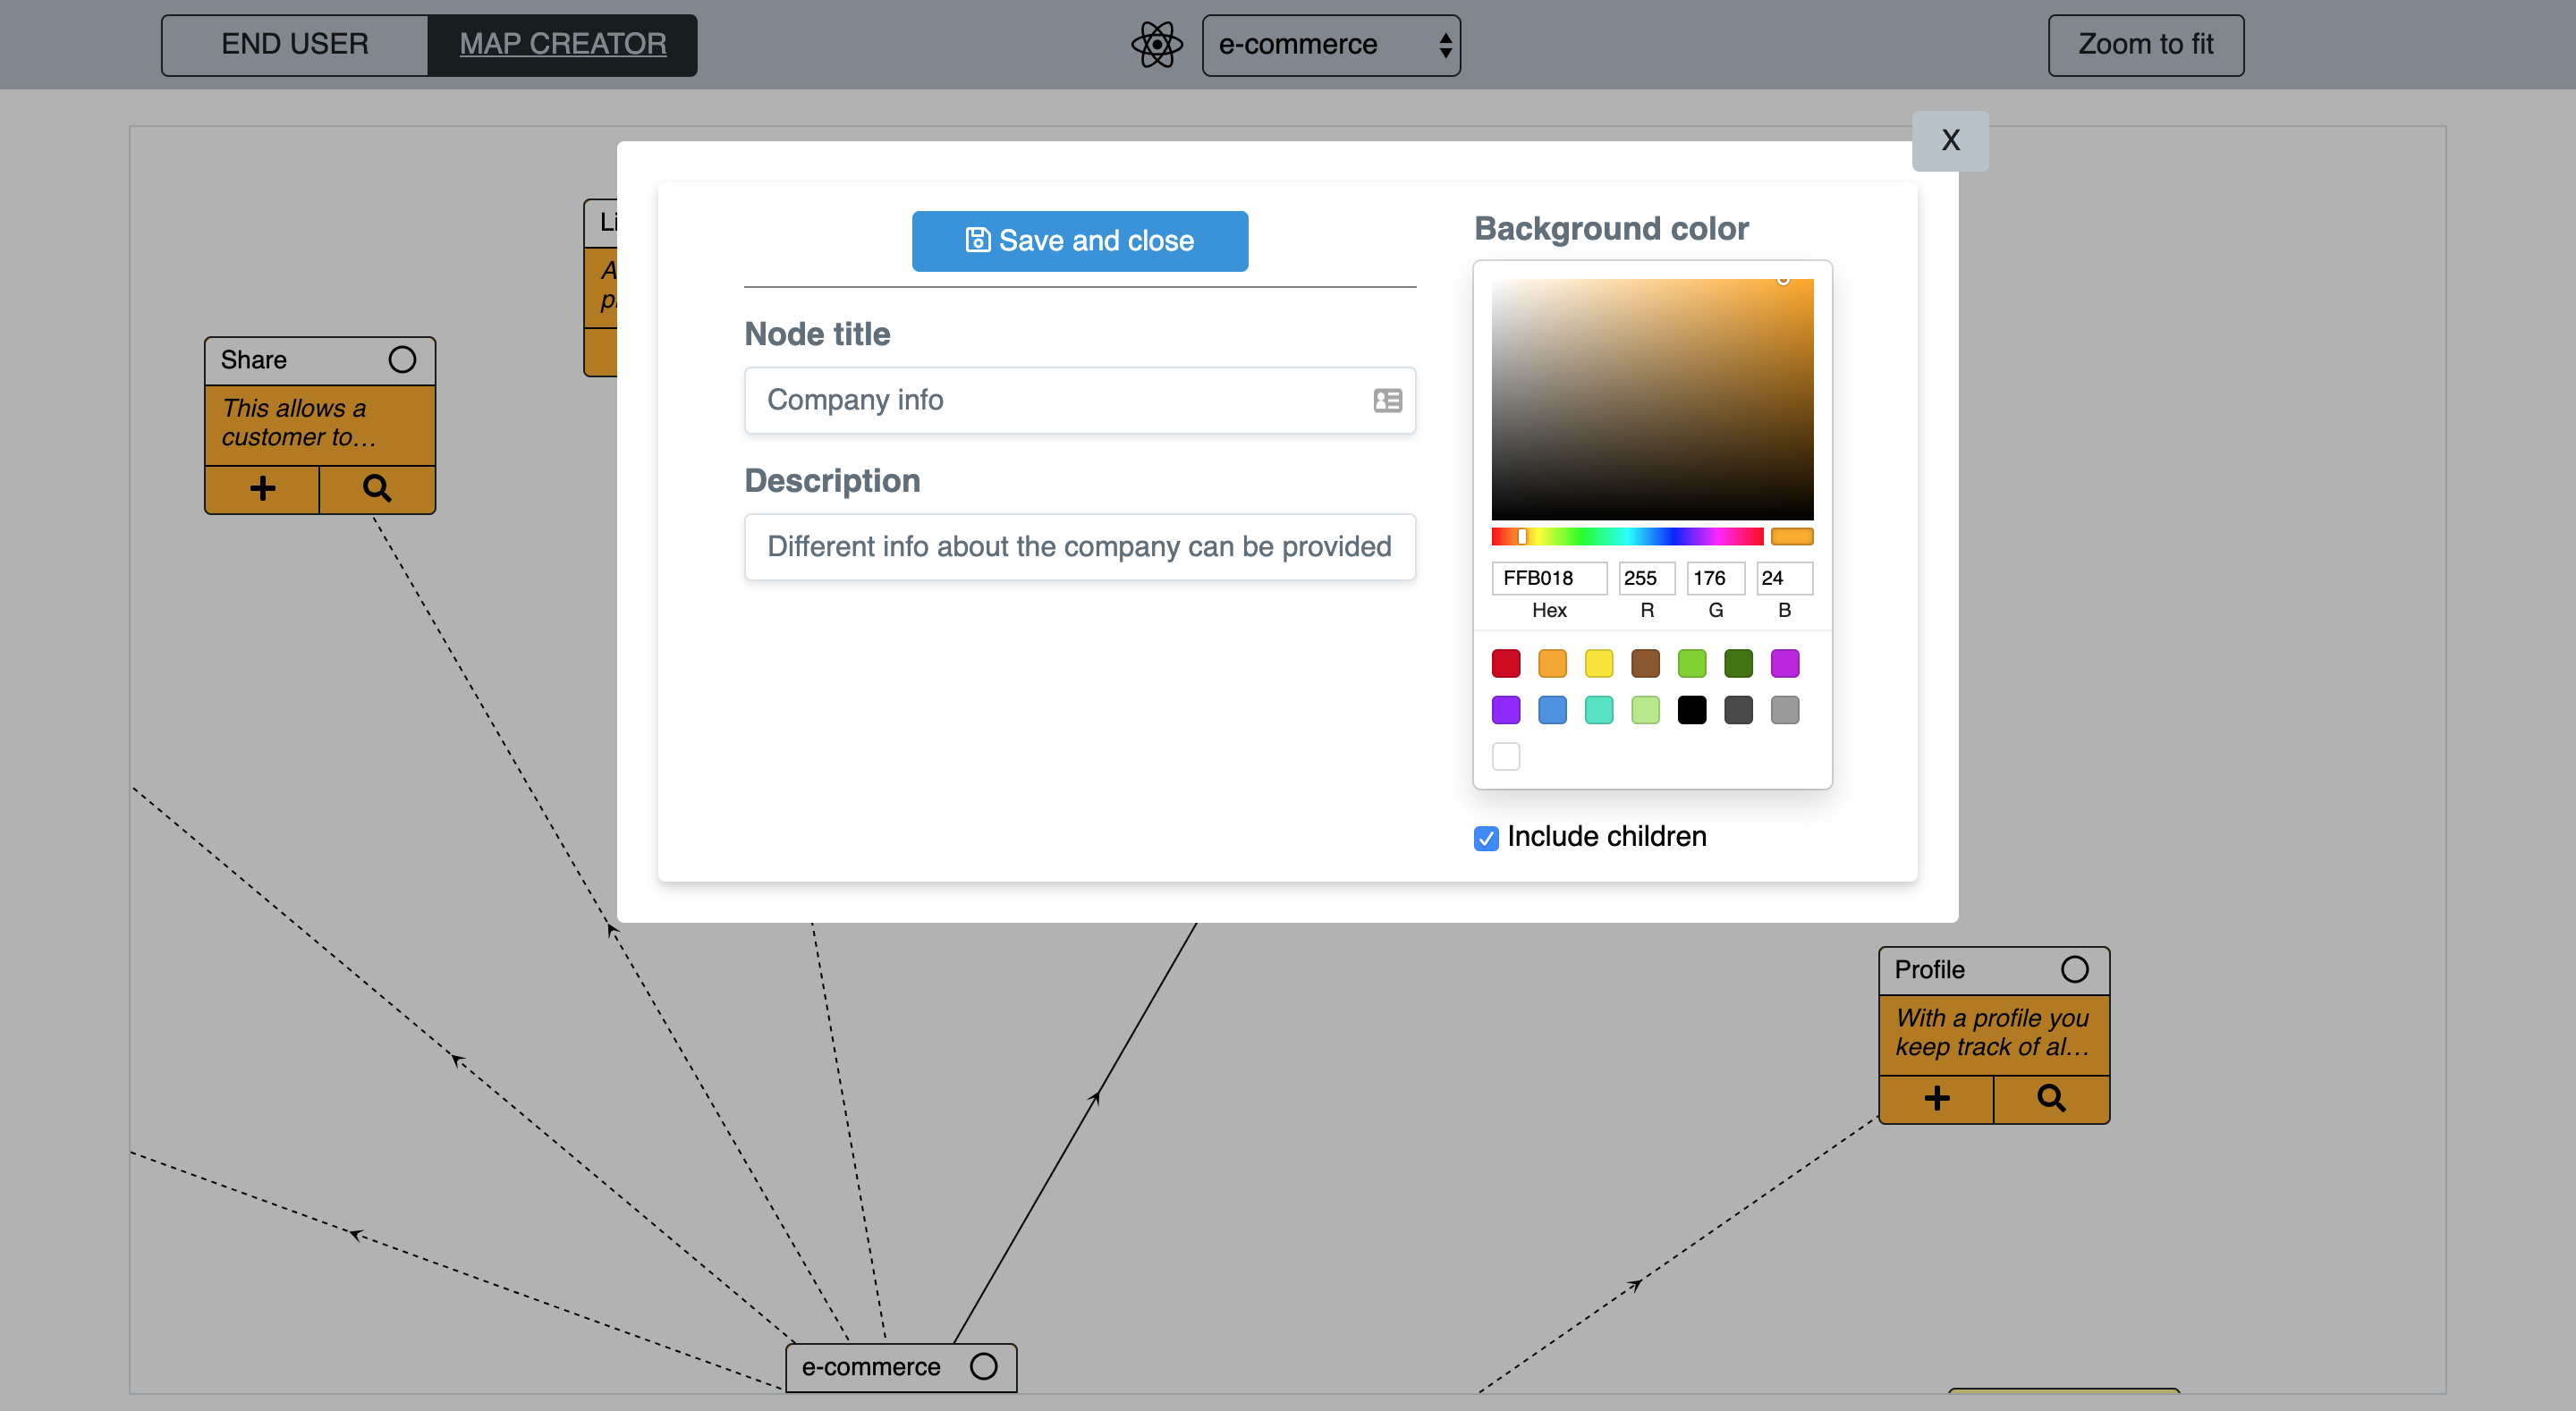
\includegraphics[width=\linewidth]{GMEditModal-MapCreator.png}}
	\caption{The edit modal in map creator mode.}
	\label{fig:gm-editmodal-mapcreator}
\end{figure}

\begin{figure}[H]
	\centering
	\frame{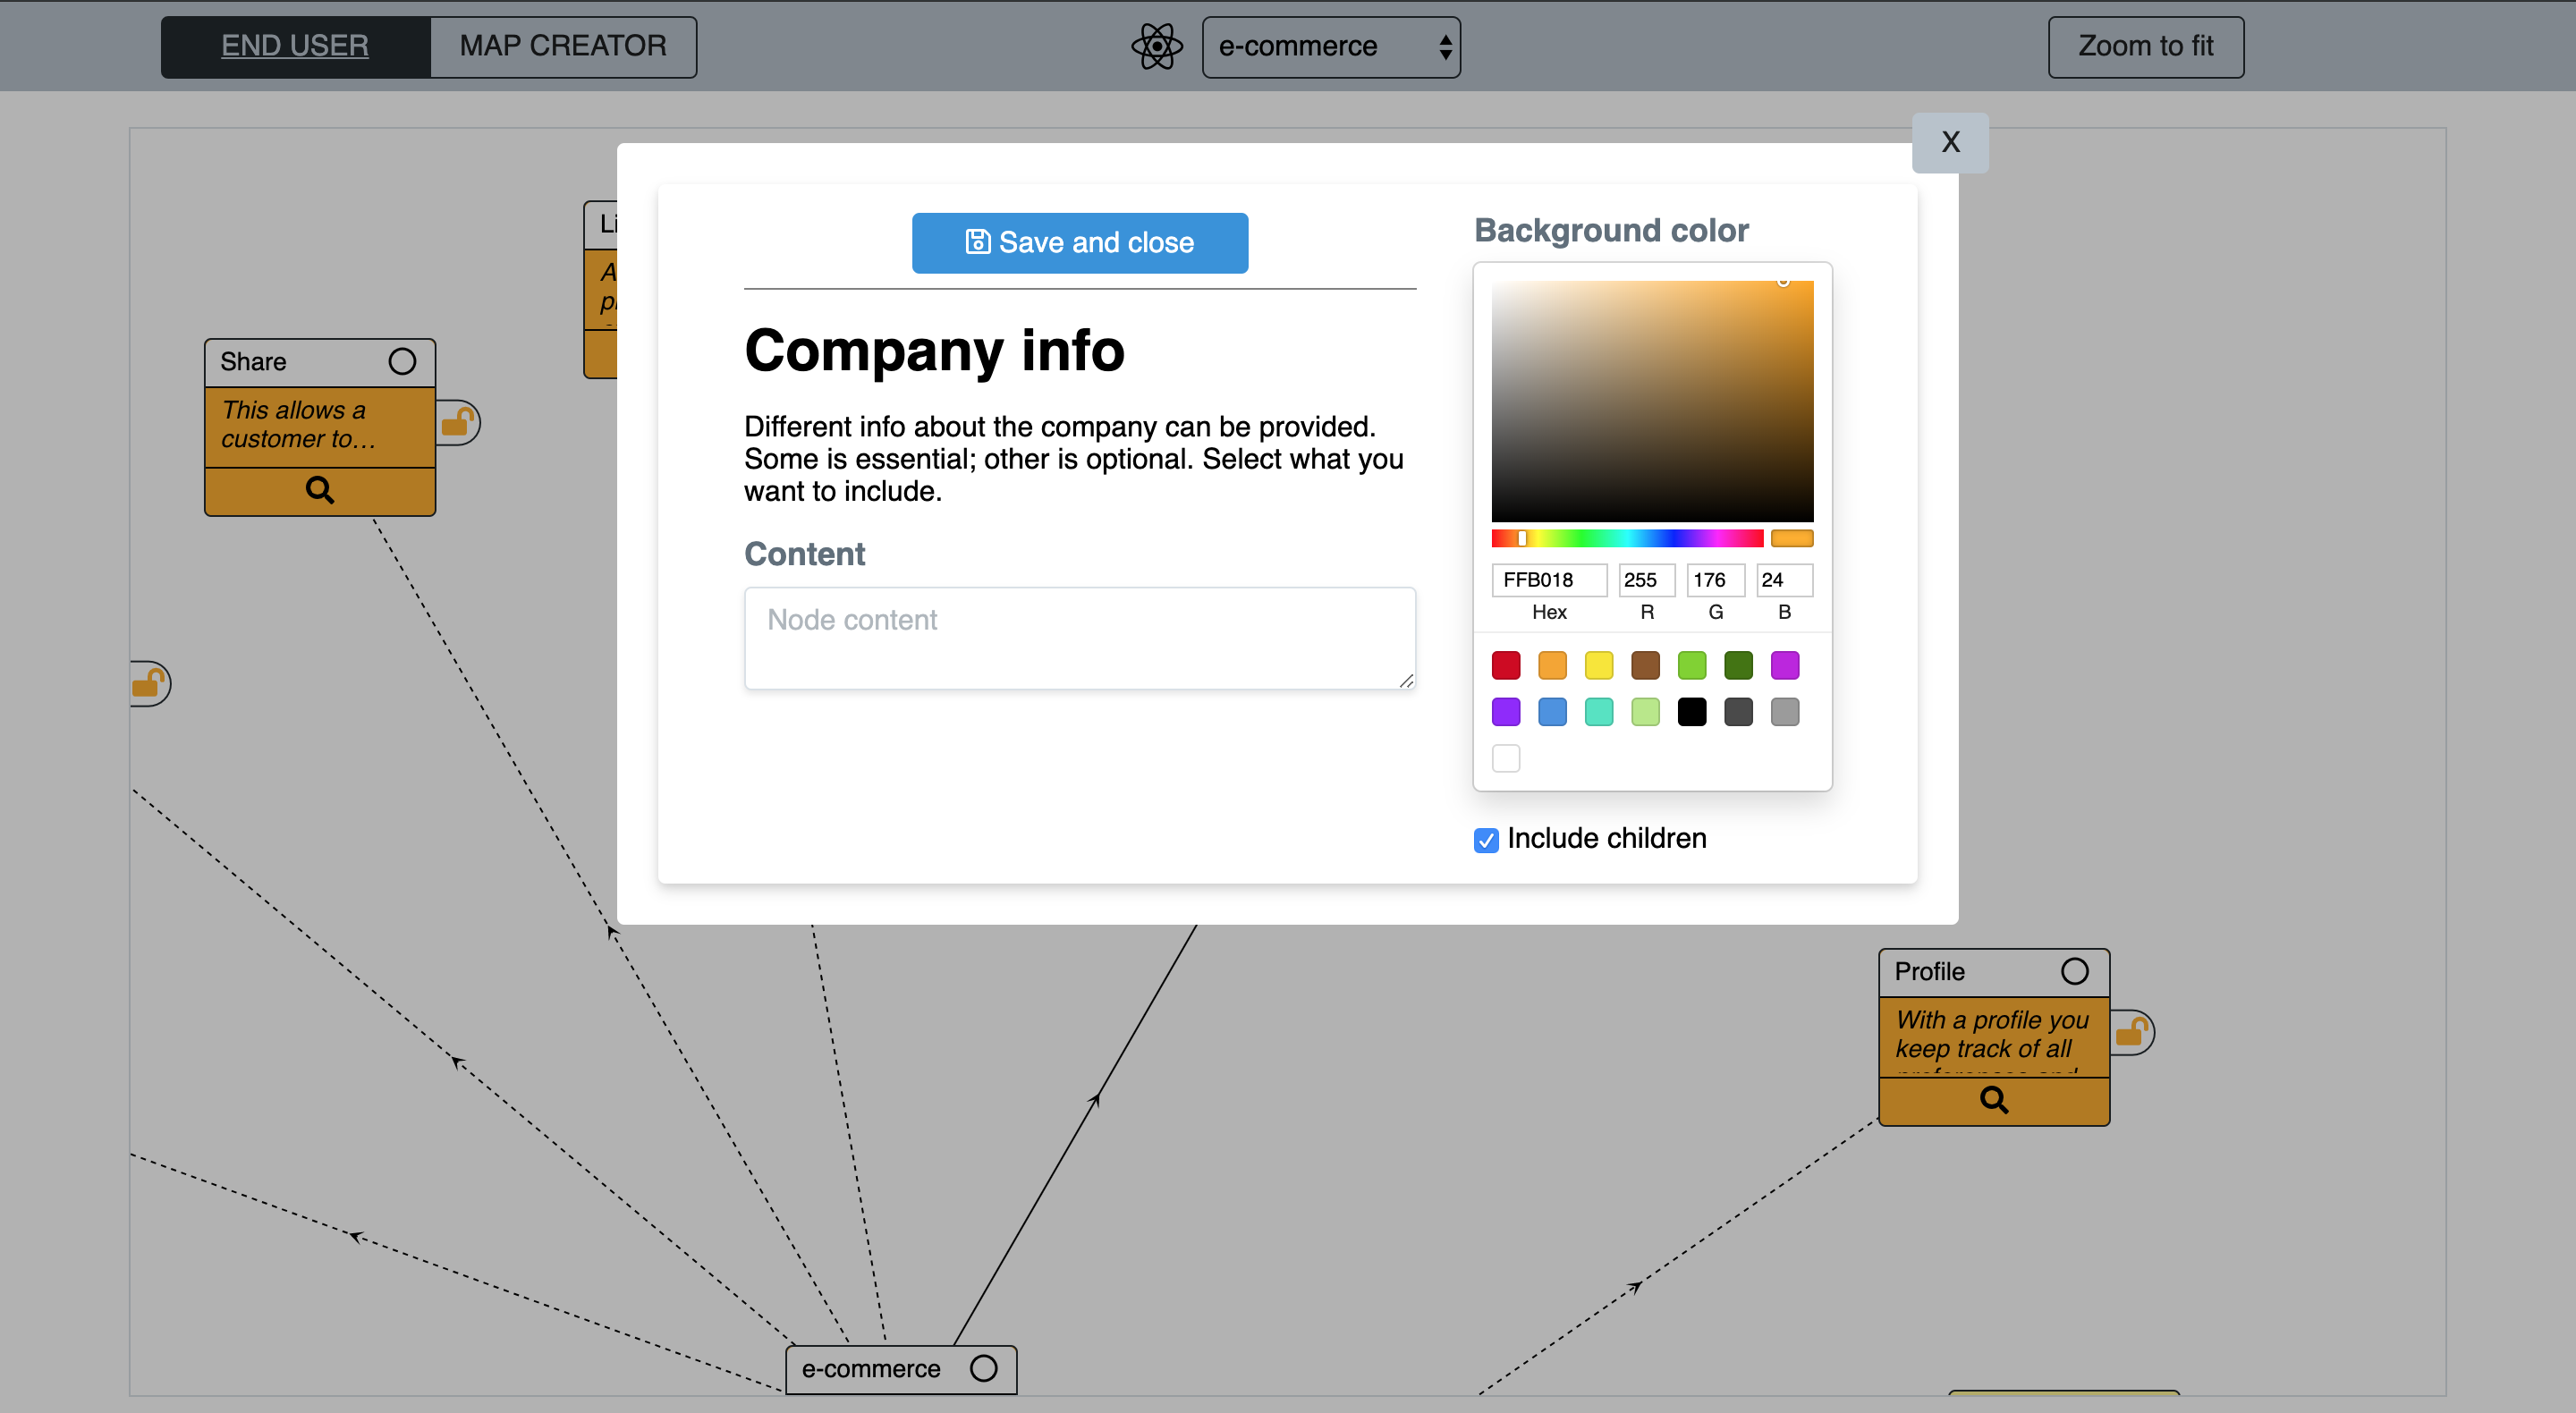
\includegraphics[width=\linewidth]{GMEditModal-EndUser.png}}
	\caption{The edit modal in end user mode.}
	\label{fig:gm-editmodal-enduser}
\end{figure}





% ----------------------------
% ------- CHOICE NODES -------
% ----------------------------
\subsection{Choice Nodes}
As explained in section \ref{sec:nodes}, choice nodes differ from the regular nodes in multiple ways. First the layout is different: while regular nodes have a title-, content- and controls-div, a choice node only has a title-div.\\

Remember that the purpose of a choice node is to let the user choose between different possibilities as children for the node. For example, the choice node with title ``Payment Method'' can have ``Cash'', ``Bancontact'' or other methods as child node. Depending on the situation, one (or more) of these methods can be chosen by the end-user.\\

It is the task of the map creator to define the possible choices the end-user can select. Therefore, when the map creator clicks on a button to add a child node, a similar modal window opens as shown in \autoref{fig:gm-add-choice}. The modal window provides text fields in which the map creator can insert a title and a description for the choice node, as well as the information for each choice, i.e. a title and a description. Because there is no maximum limit on the number of choices a map creator can provide, he can always ask to add more text fields to be able to give the information about an additional choice.\\

Another feature particular for choice nodes consists of the cardinalities a map creator can define. The map creator can set a lower limit and an upper limit. The lower limit is the minimum number of choices the end-user has to select. For example, if the lower limit is equal to two, the end-user cannot select only one choice. The upper limit is the maximum number of choices that can be selected by the end-user. By default the lower limit is equal to zero and the upper limit is equal to the total number of choices the map creator provided. It is not possible to set the upper limit equal to zero because this would not make sense: end-user would not be able to select any choice. Hence, the choice node would have no meaning and be useless.

\begin{figure}[H]
	\centering
	\frame{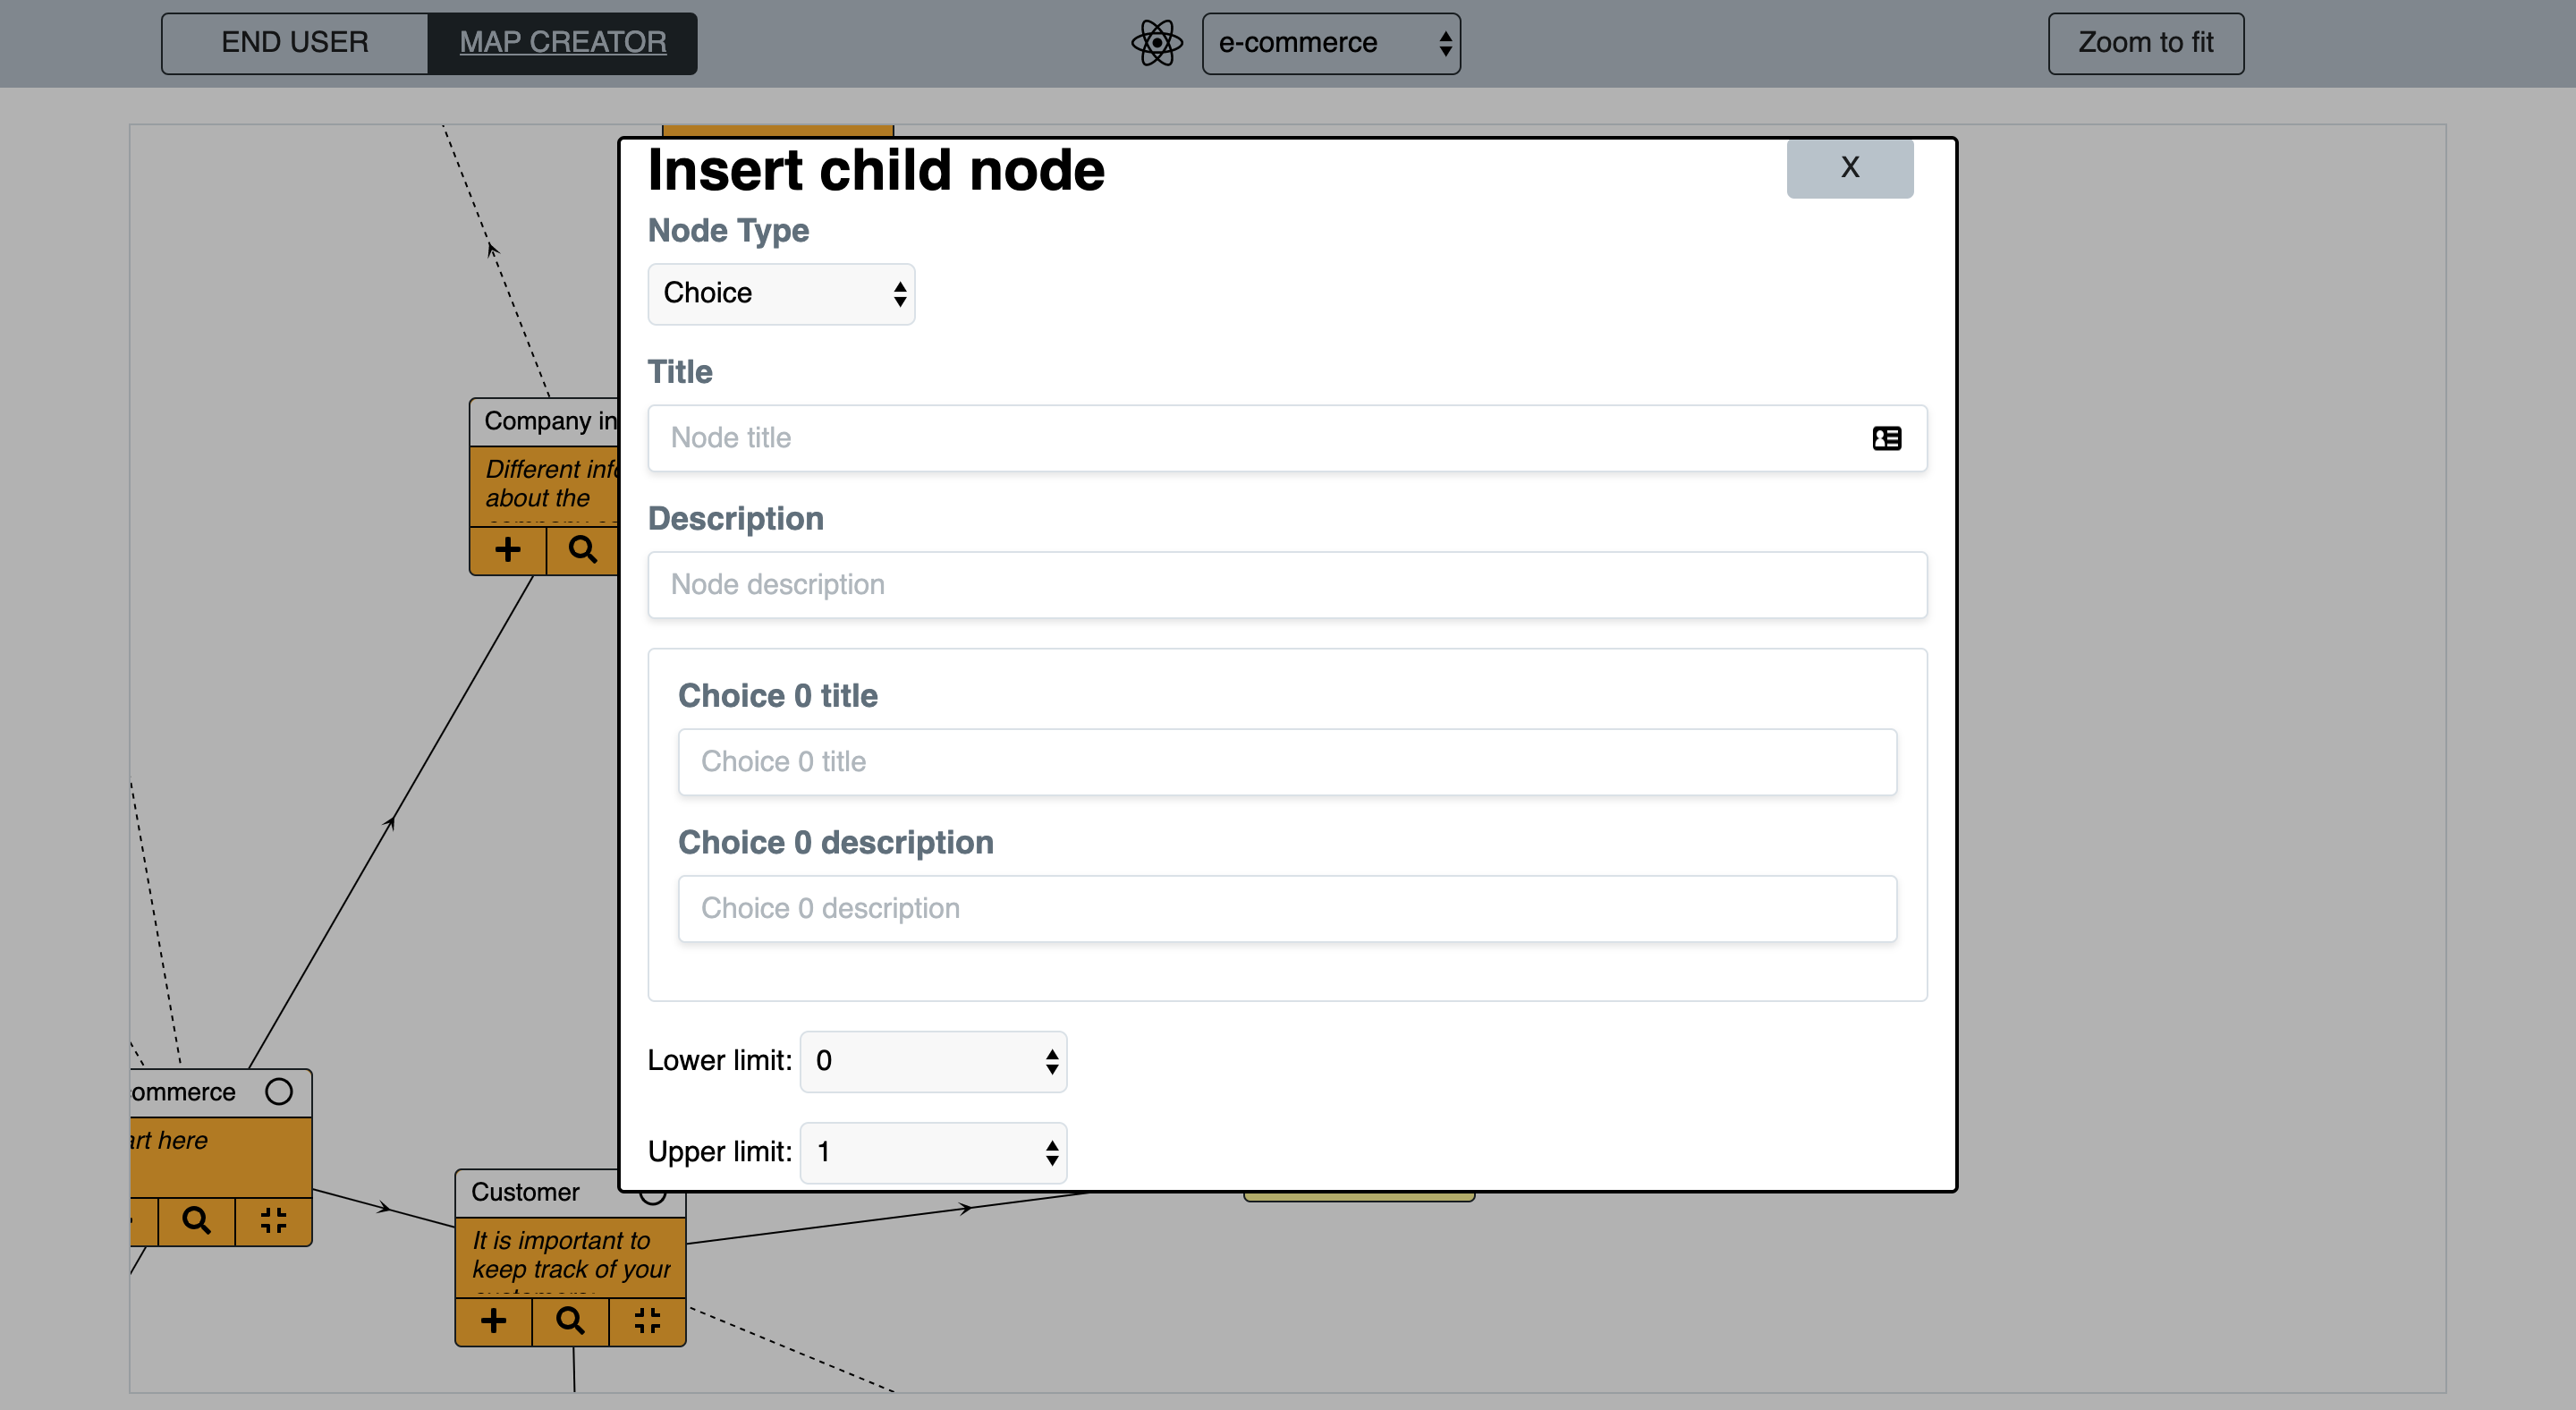
\includegraphics[width=\linewidth]{GMAddChildNodeModal-Choice.png}}
	\caption{Adding a choice node.}
	\label{fig:gm-add-choice}
\end{figure}

After the node is created, the map creator can edit the node by performing a single click on the choice node. Then a modal window opens and he can edit the title, the description and the already defined choices (see \autoref{fig:gm-choicenode-mapcreator}). To delete a choice, the map creator only has to empty the text fields of the choice.

\begin{figure}[H]
	\centering
	\frame{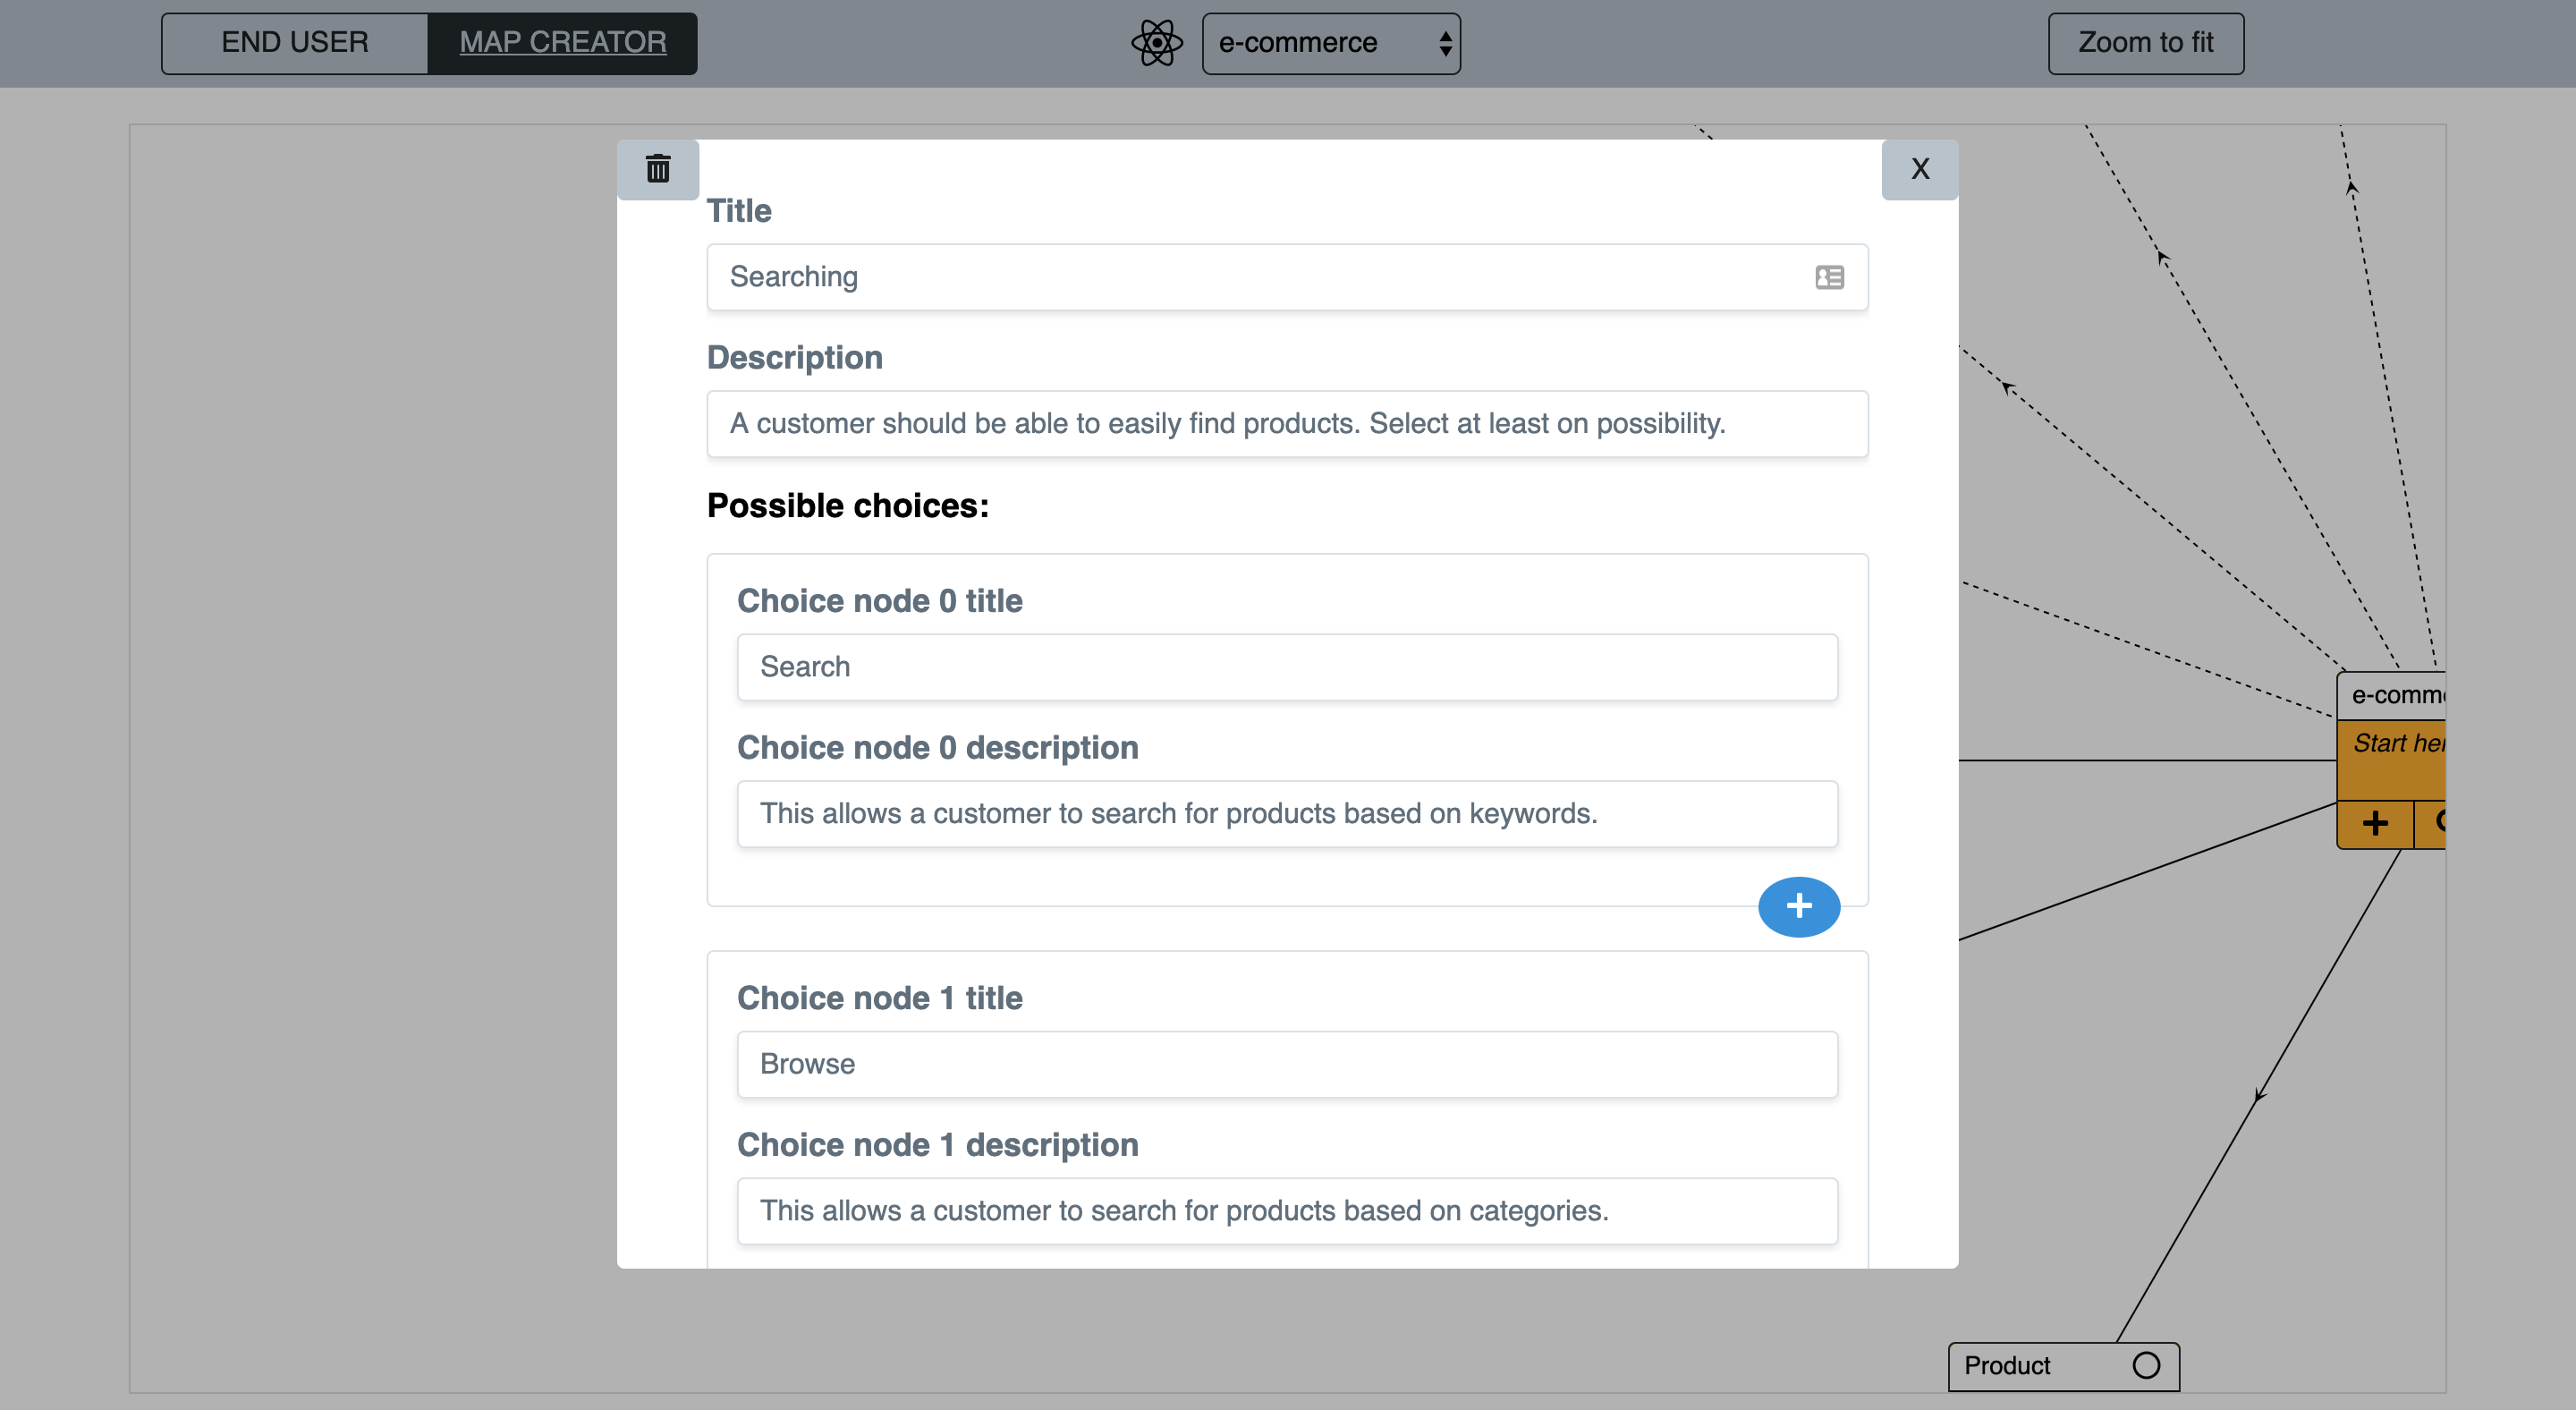
\includegraphics[width=\linewidth]{GMChoiceNode-MapCreator.png}}
	\caption{An opened choice node in map creator mode.}
	\label{fig:gm-choicenode-mapcreator}
\end{figure}

The modal window showing up when the end-user clicks on a choice node (see \autoref{fig:gm-choicenode-enduser}) is not equal to the modal window the map creator can see after the same action. The end-user sees the title and description of the node on top, but (s)he cannot edit these like a map creator. Under the description is shown how many choices the end-user should select. For example ``Select between 1 and 3 choices'', where 1 is the lower limit and 3 the upper limit set by the map creator. This instruction is followed by a form, where every possible choice is made visible by showing the title and the description. The end-user can select the choices he wants via a checkbox. With a click on the button, the selected choices are registered and added as children to the choice node. It is possible at any time to adapt the choices by reopening the modal window. At that moment, the checkbox(es) of the previously selected choice(s) will be checked. To remove a choice as child of the choice node, it is sufficient to uncheck the checkbox.\\

Next to selecting choices given by the map creator, it can sometimes be necessary to be able to add an extra possibility, which was not given by the map creator. Therefore, an end-user can create additional choices, which he can select later on. Additional choices can be created in the same way as the map creator can do it. By a click on the button, an additional part of the form appears in the modal window. When the form is submitted, the additional choice is registered with the given title and description. An example is shown in \autoref{fig:gm-choicenode-enduser-extraoption}.
\begin{figure}[H]
	\centering
	\frame{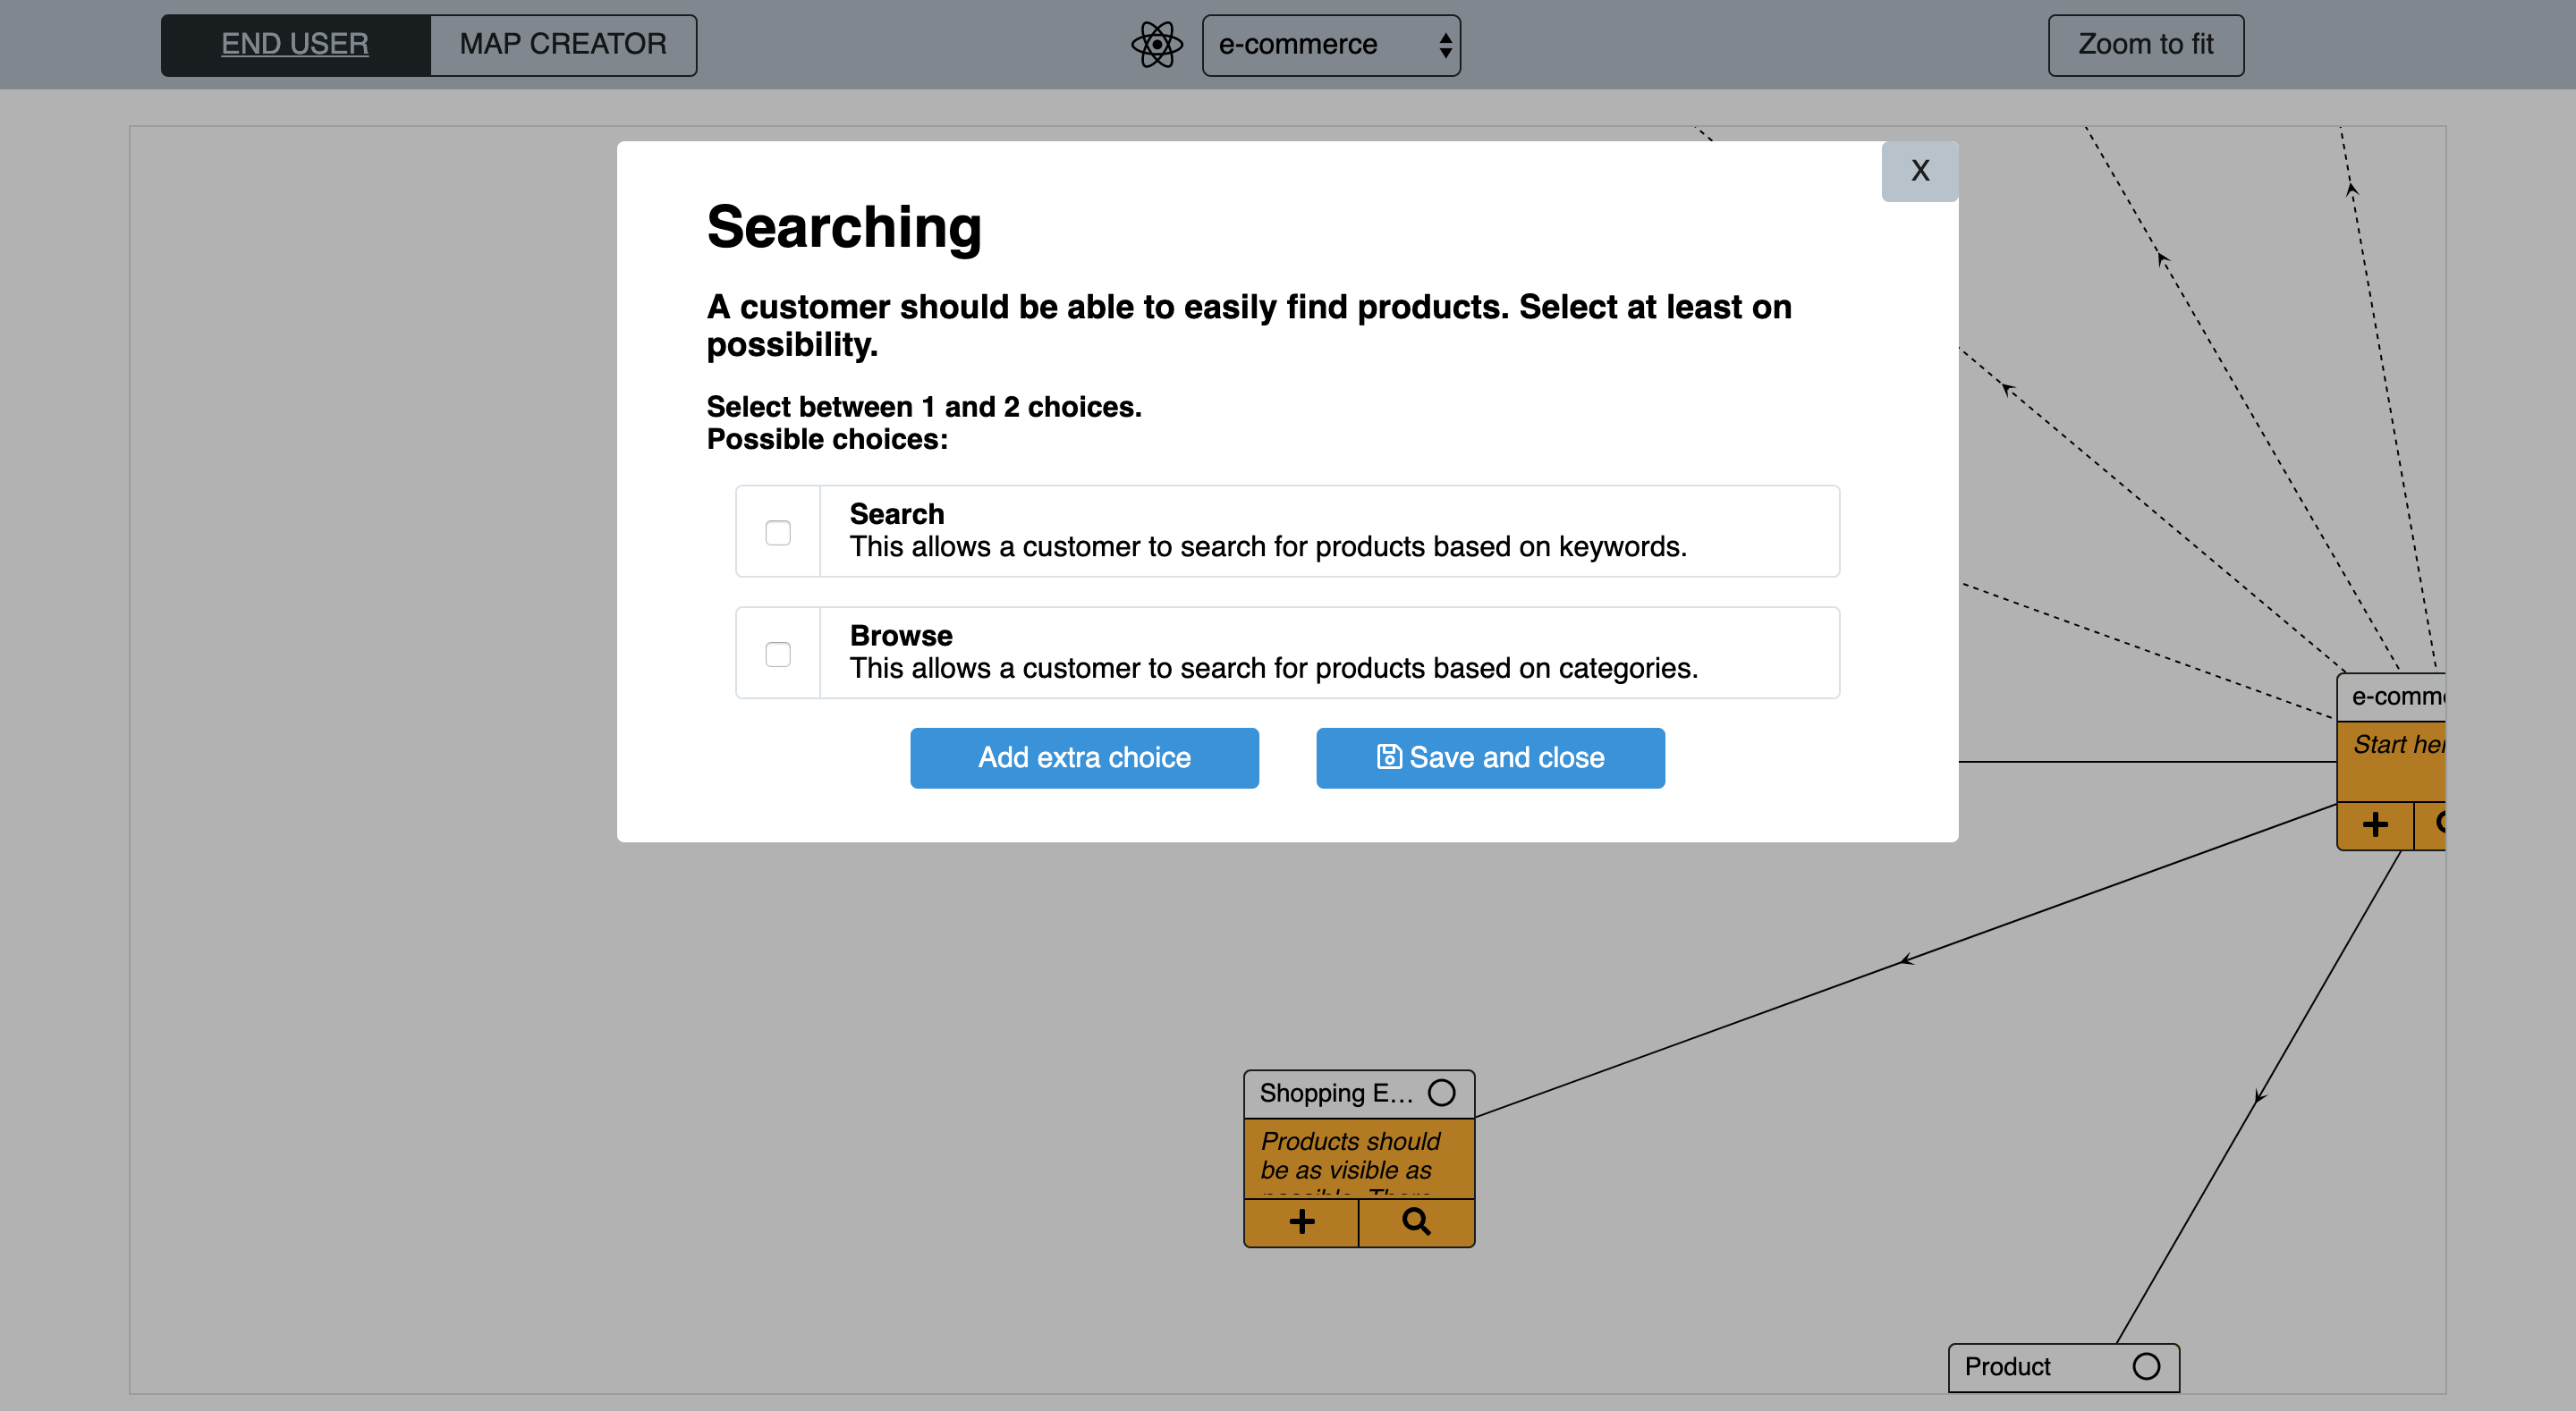
\includegraphics[width=\linewidth]{GMChoiceNode-EndUser.png}}
	\caption{An opened choice node in end user mode.}
	\label{fig:gm-choicenode-enduser}
\end{figure}

\begin{figure}[H]
	\centering
	\frame{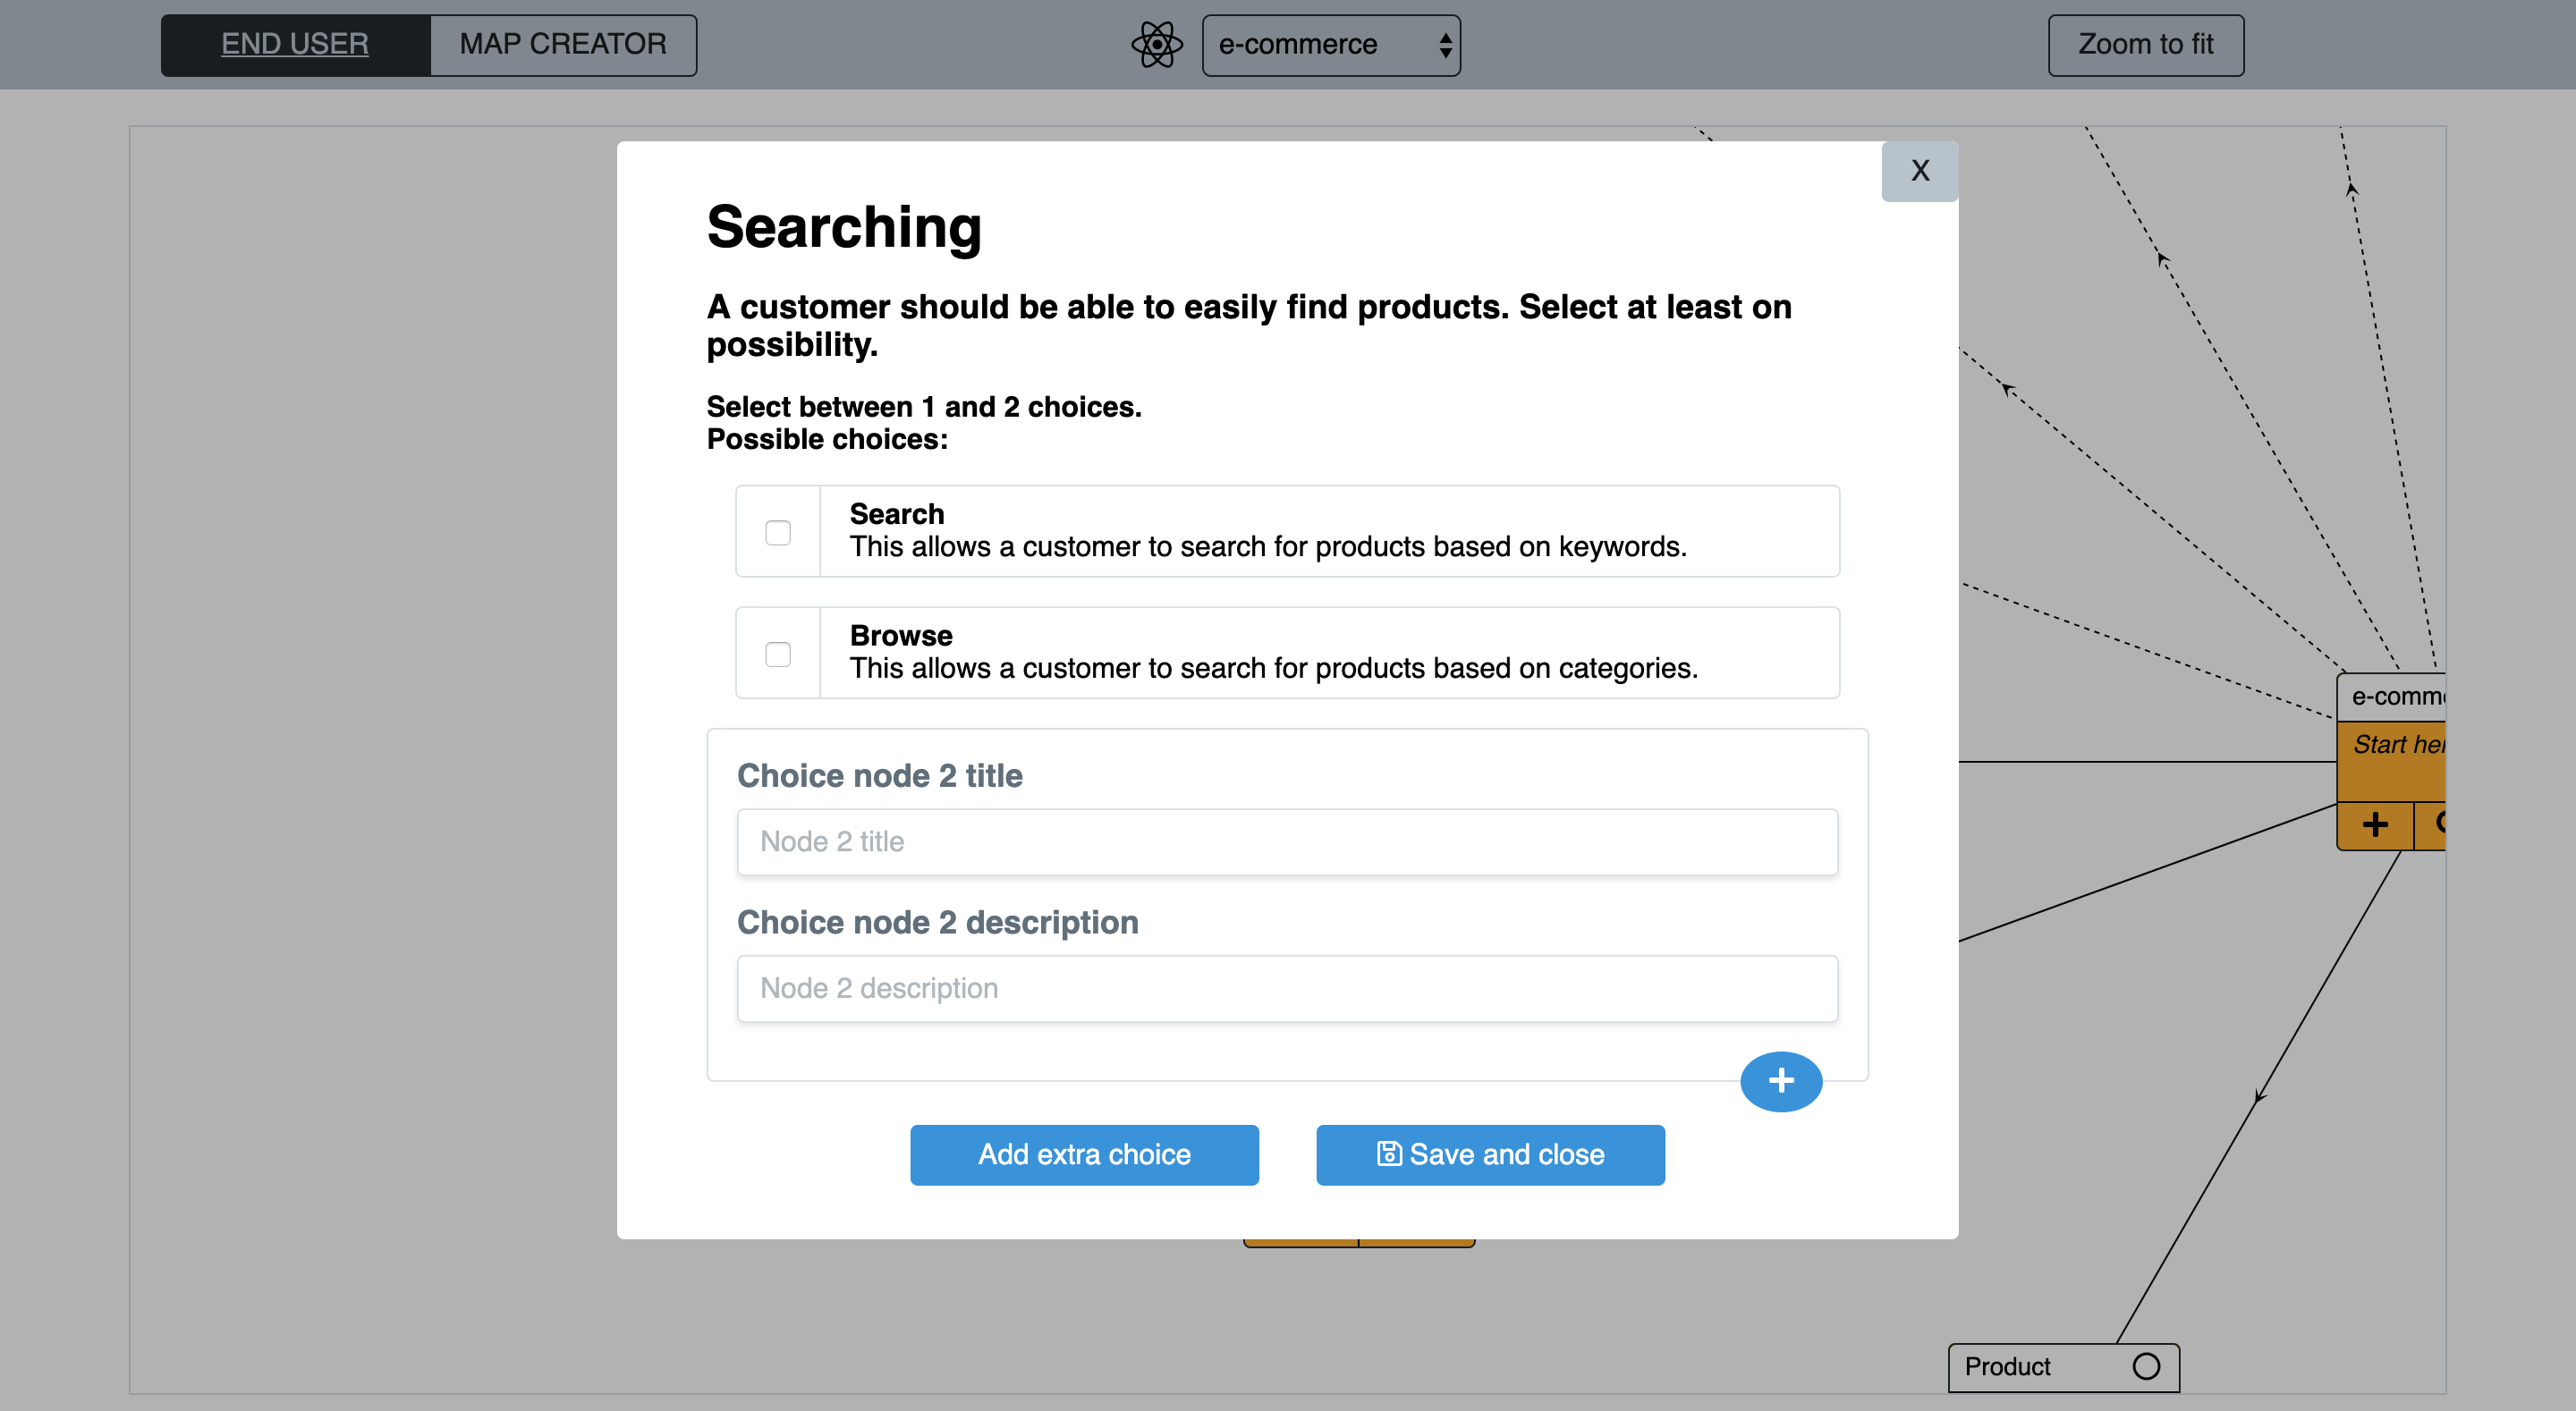
\includegraphics[width=\linewidth]{GMChoiceNode-EndUser-ExtraOption.png}}
	\caption{An opened choice node in end user mode with option to select additional choice.}
	\label{fig:gm-choicenode-enduser-extraoption}
\end{figure}



% ----------------------------
% ------ OPTIONAL NODES ------
% ----------------------------
\subsection{Optional nodes}\label{sec:optional-nodes}
A map can also provide optional nodes. They can be recognized by the dotted link between this node and its parent. A special characteristic of optional nodes is that these nodes can be disabled by the end-user. Therefore, optional nodes contain an additional button, represented as a lock, at their right side. As long as the node is enabled, the button is represented by an open lock. A click on this button disables the node and changes the icon into a closed lock. The node can be enabled again by clicking the lock again. Next to the lock icon, a disabled node can be recognized by its gray background and a blurred content so that the content is less readable.\\

A second characteristic of optional nodes is that they do not contribute to the ``completeness icon'' of the visualization. Hence, to determine whether the completeness icon of a node should be empty, filled or partially filled, optional child nodes and their descendants (which are optional as well) are skipped because it does not matter whether content is provided in these nodes or not. There is only one exception on this rule: when a choice node is optional but it does have children (selected by the end-user), these children are not optional and are checked for completeness.















\clearpage

\chapter{Another Use Case}\label{ch:usecase}
To demonstrate that we achieved \ref{goal:generic}, we implemented a different use case for the system called \textit{Plateforme DD (PDD)}. In the first section of this chapter, we describe the purpose of this use case and explain Plateforme DD. The second section is about how the library could be used to create a visualization for this system.

\section{Plateforme DD}\label{sec:pdd}
PDD is a ULB (Universit\'e Libre de Bruxelles) project with a scientific mission, i.e. durable development in Brussels. On the one hand, the project tries to arouse interest in sciences among pupils in Brussels. On the other hand, it wants to make it easier (for everyone, not only pupils) to understand the situation in Brussels and to make them take efforts for a durable development in the city.\\

The different pages on the website\footnote{https://sciences.brussels/dd/} of Plateforme DD correspond to projects the pupils worked on in small groups. The content on every page can be seen as a small report concerning what they learned about the topic. Many of these topics are linked to each other in some way. However, it is absolutely not easy to understand the underlying tree structure by browsing through the website. On each page corresponding to one of the topics, a number of links can be found. But by following these links, the user can get lost quite easily on this site and it is very difficult to understand how the different projects are linked to each other. Hence, the project owners wanted to have a better visualization of the relationships between the different Web pages. Therefore, we visualized the tree structure by creating a separate node for each (sub)topic on the site. In this way, it should be easier for the user to grasp the relationships between the different projects. To create such a visualization, we could make use of our library. In this way, we can show that our tool can be used in cases where the visualization and functionality is completely different from the one for GuideaMaps. The created visualization for the content of the Plateforme DD website can be seen in \autoref{fig:plateforme-dd}.


\begin{figure}[H]
	\centering
	\frame{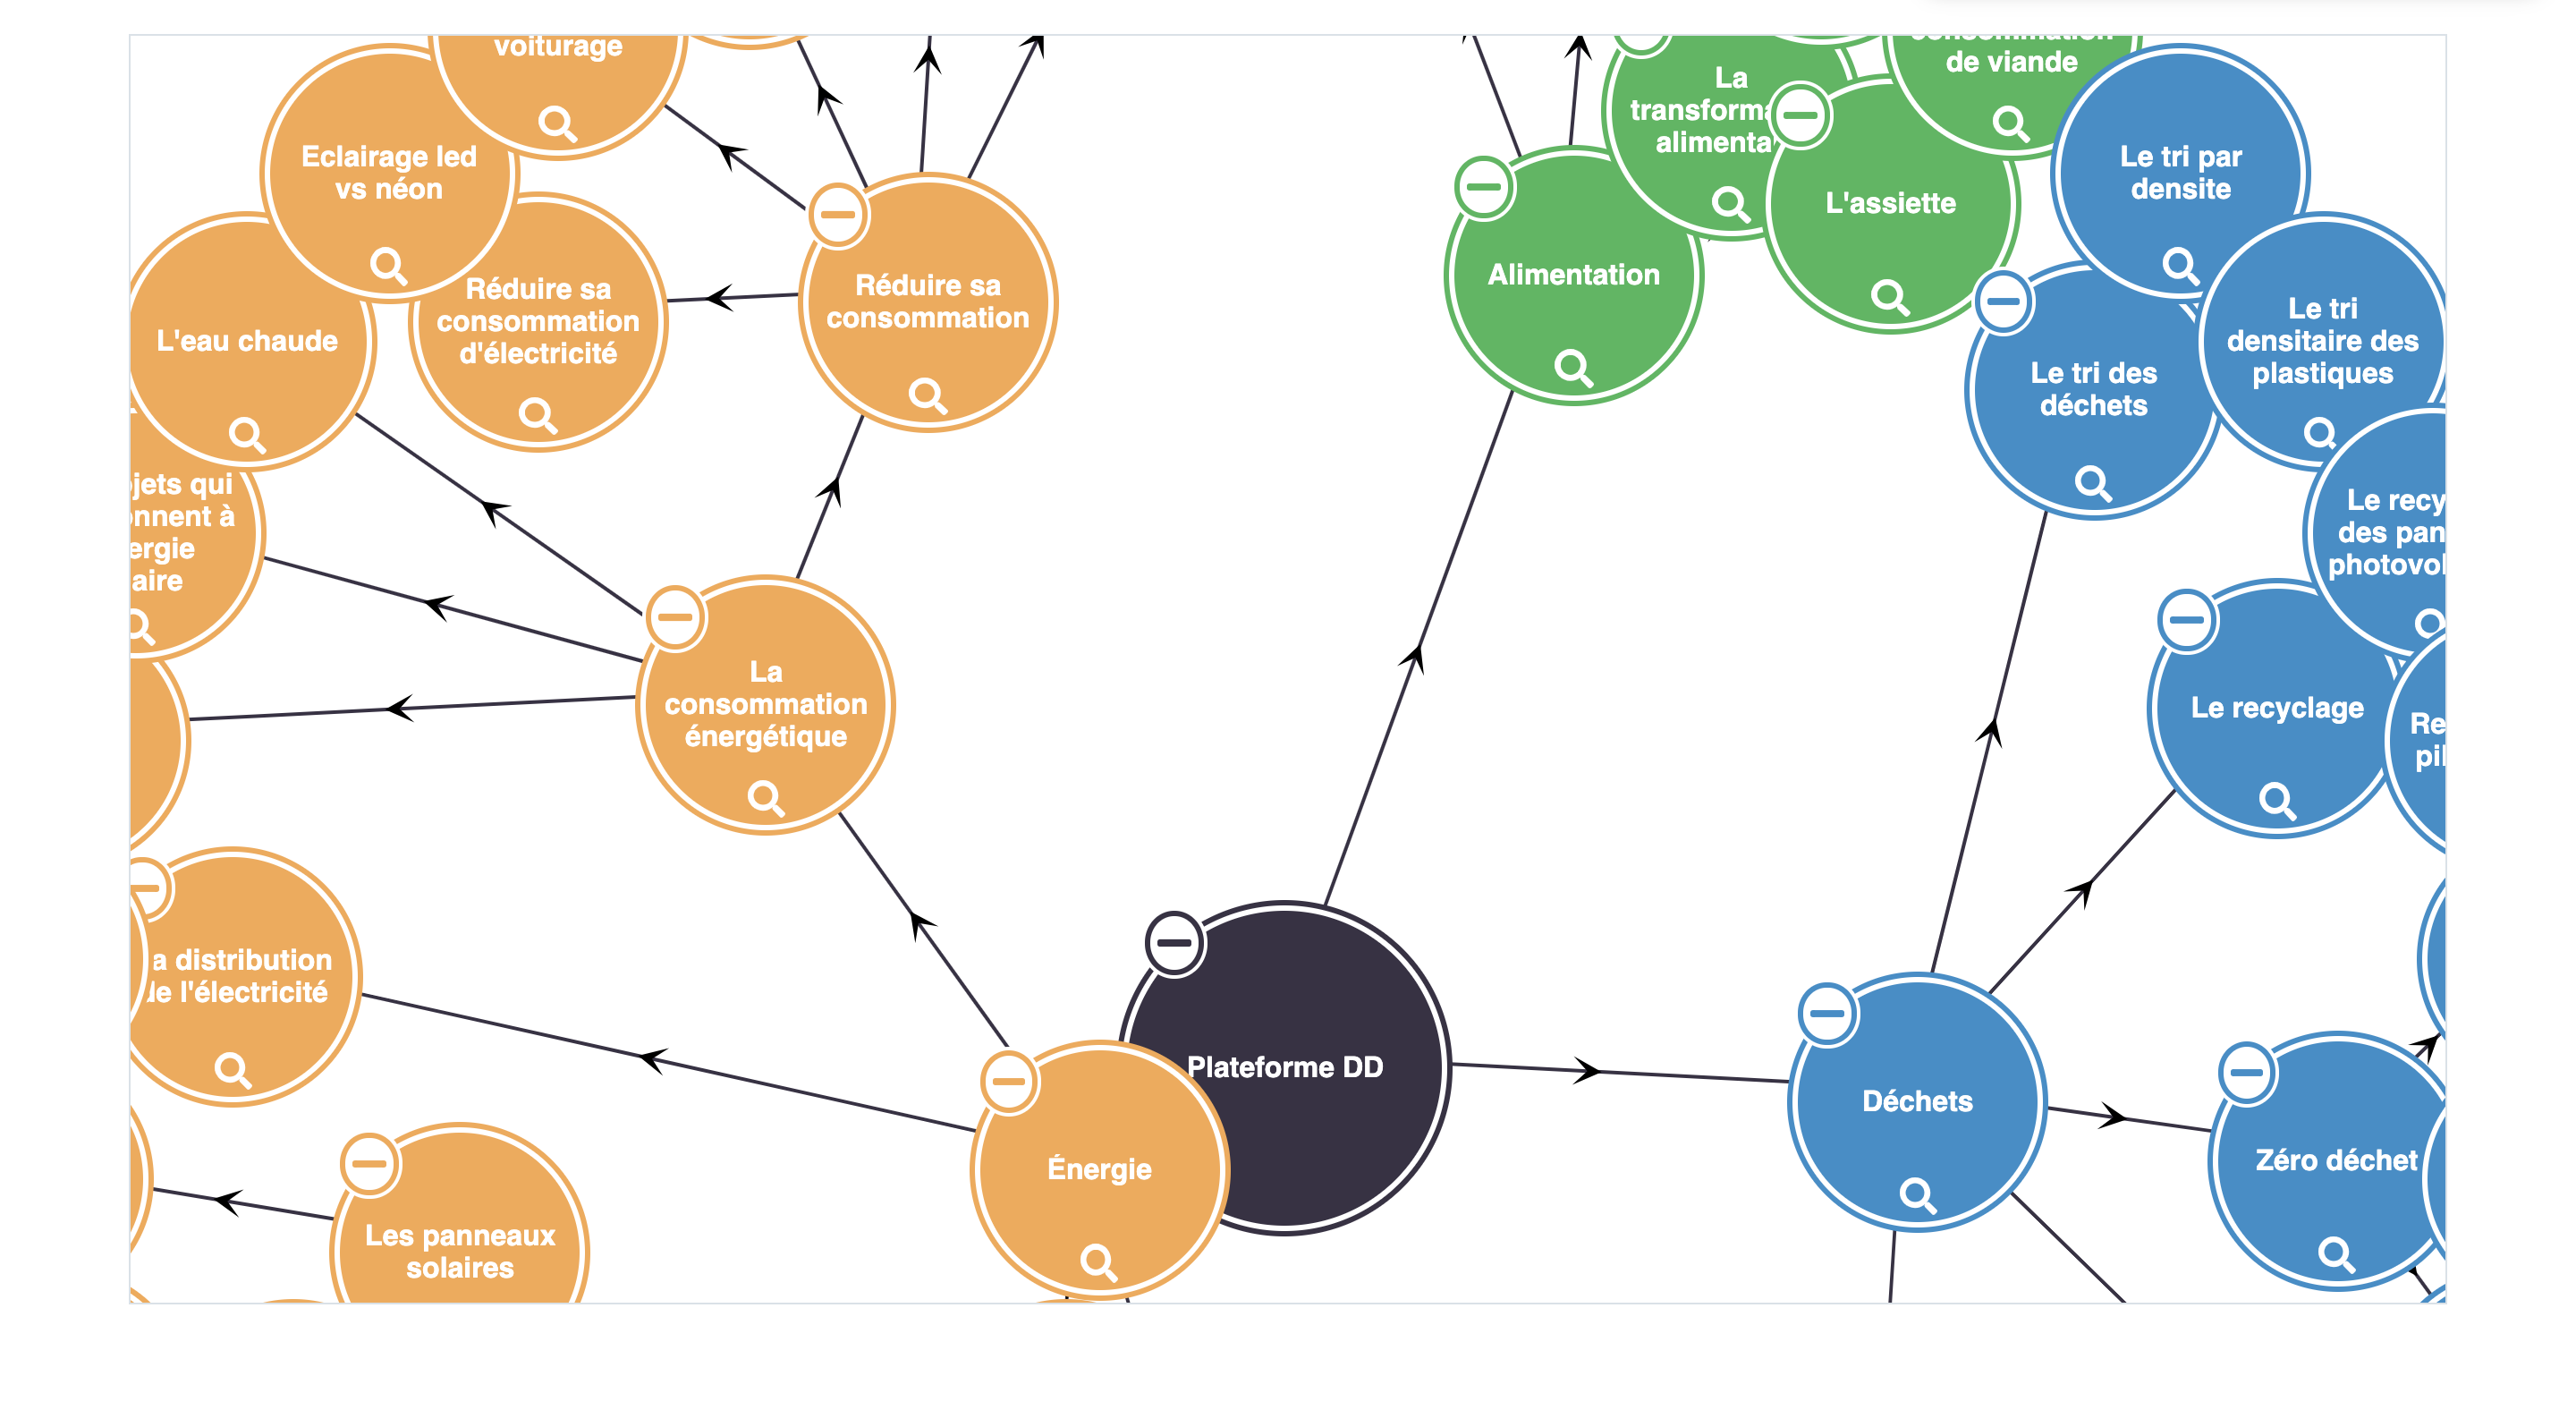
\includegraphics[width=\linewidth]{usecase/plateforme-dd.png}}
	\caption{Plateforme DD Visualization.}
	\label{fig:plateforme-dd}
\end{figure}



\section{Customization Effort}\label{sec:customization-effort}
In \autoref{fig:examplecode-library}, we showed how we could alter the visualization of the data without affecting the default code. Remember that the props in that figure are not the only customizable props of the library. \autoref{fig:differences-gm-vs-pdd} shows the differences in configuration when we compare the visualization of GuideaMaps with the one of Plateforme DD.

\begin{figure}[H]
	\begin{minipage}{0.5\textwidth}
 		 \centering
		 \begin{minted}[breaklines, linenos, escapeinside=||]{html}
<ZoomableTree
    |\textcolor{mygreen}{NodeComp}|=|\textcolor{red}{\{GMNode\}}|
    |\textcolor{mygreen}{LinkComp}|=|\textcolor{red}{\{GMLink\}}|
    |\textcolor{mygreen}{EditModalComp}|=|\textcolor{red}{\{ GMEditModal\}}|
    |\textcolor{mygreen}{onAddNode}|=|\textcolor{red}{\{addGMNode\}}|
    |\textcolor{mygreen}{onDeleteNode}|=|\textcolor{red}{\{ deleteGMNode\}}|
    |\textcolor{mygreen}{onNodeUpdate}|=|\textcolor{red}{\{args -> updateGMNode(args)\}}|
    |\textcolor{mygreen}{onVisibleChildrenUpdate}|=|\textcolor{red}{\{ nodeId => updateGMVisibleChildren( nodeId)\}}|
/>
		\end{minted}
		\label{lst:default-components}
		\captionof{lstlisting}{GM Configuration.}
	\end{minipage}
 	\begin{minipage}{0.5\textwidth}
  		\centering
  		\begin{minted}[breaklines, escapeinside=||]{html}
<ZoomableTree
    |\textcolor{mygreen}{NodeComp}|=|\textcolor{red}{\{PDDNode\}}|
    |\textcolor{mygreen}{LinkComp}|=|\textcolor{red}{\{PDDLink\}}|
    |\textcolor{mygreen}{EditModalComp}|=|\textcolor{red}{\{ PDDEditModal\}}|
    |\textcolor{mygreen}{onAddNode}|=|\textcolor{red}{\{() -> null\}}|
    |\textcolor{mygreen}{onDeleteNode}|=|\textcolor{red}{\{ deleteGMNode\}}|
    |\textcolor{mygreen}{onNodeUpdate}|=|\textcolor{red}{\{args -> updateGMNode(args)\}}|
    |\textcolor{mygreen}{onVisibleChildrenUpdate}|=|\textcolor{red}{\{ nodeId => updateGMVisibleChildren( nodeId)\}}|
/>
		\end{minted}
		\label{lst:custom-components}
 	 	\captionof{lstlisting}{PDD Configuration.}
 	\end{minipage}
	\caption{The configuration differences between GuideaMaps and Plateforme DD.}
	\label{fig:differences-gm-vs-pdd}
 	%\captionof{figure}{Two listings showing the difference between the default and custom use of the library.}
\end{figure}

\subsection{NodeComp}\label{sec:usecase-nodecomp}
The most obvious difference, which can immediately be seen when comparing both visualizations, is the layout of the nodes. In GuideaMaps (GM), we had rectangular nodes, while in Plateforme DD (PDD) the nodes are circular. To achieve this result, we implemented a special component, called \textit{PDDNode}, to replace \textit{GMNode}. From then on, every node in the data will be visualized by the code of PDDNode instead of the code of GMNode. Hence, GMNode still exists; it is not deleted or overwritten, but simply not used in this configuration.



\subsection{LinkComp}\label{sec:usecase-linkcomp}
The second prop is responsible for the representation of the links. You will not observe big differences between a GMLink and a PDDLink, except for the thickness: a PDDLink is thicker than a GMNode. As a consequence, the implementation of PDDLink is a copy of the GMLink with the value for \textit{strokeWidth} as only difference. \\

If the user does not need a different style for the links, he does not have to create a PDDLink component. In that case, it is possible to use GMLink as LinkComp, while the other props are eventually specially created for Plateforme DD.



\subsection{EditModalComp}\label{sec:usecase-editmodalcomp}
The edit modal of Plateforme DD is completely different compared to the one of GuideaMaps. First of all, it is not a real \textit{edit}-modal because a user of the PDD visualization is not allowed to update the data of the nodes, he can only consult the available data, represented as in \autoref{fig:pdd-editmodal}.

\begin{figure}[H]
	\centering
	\frame{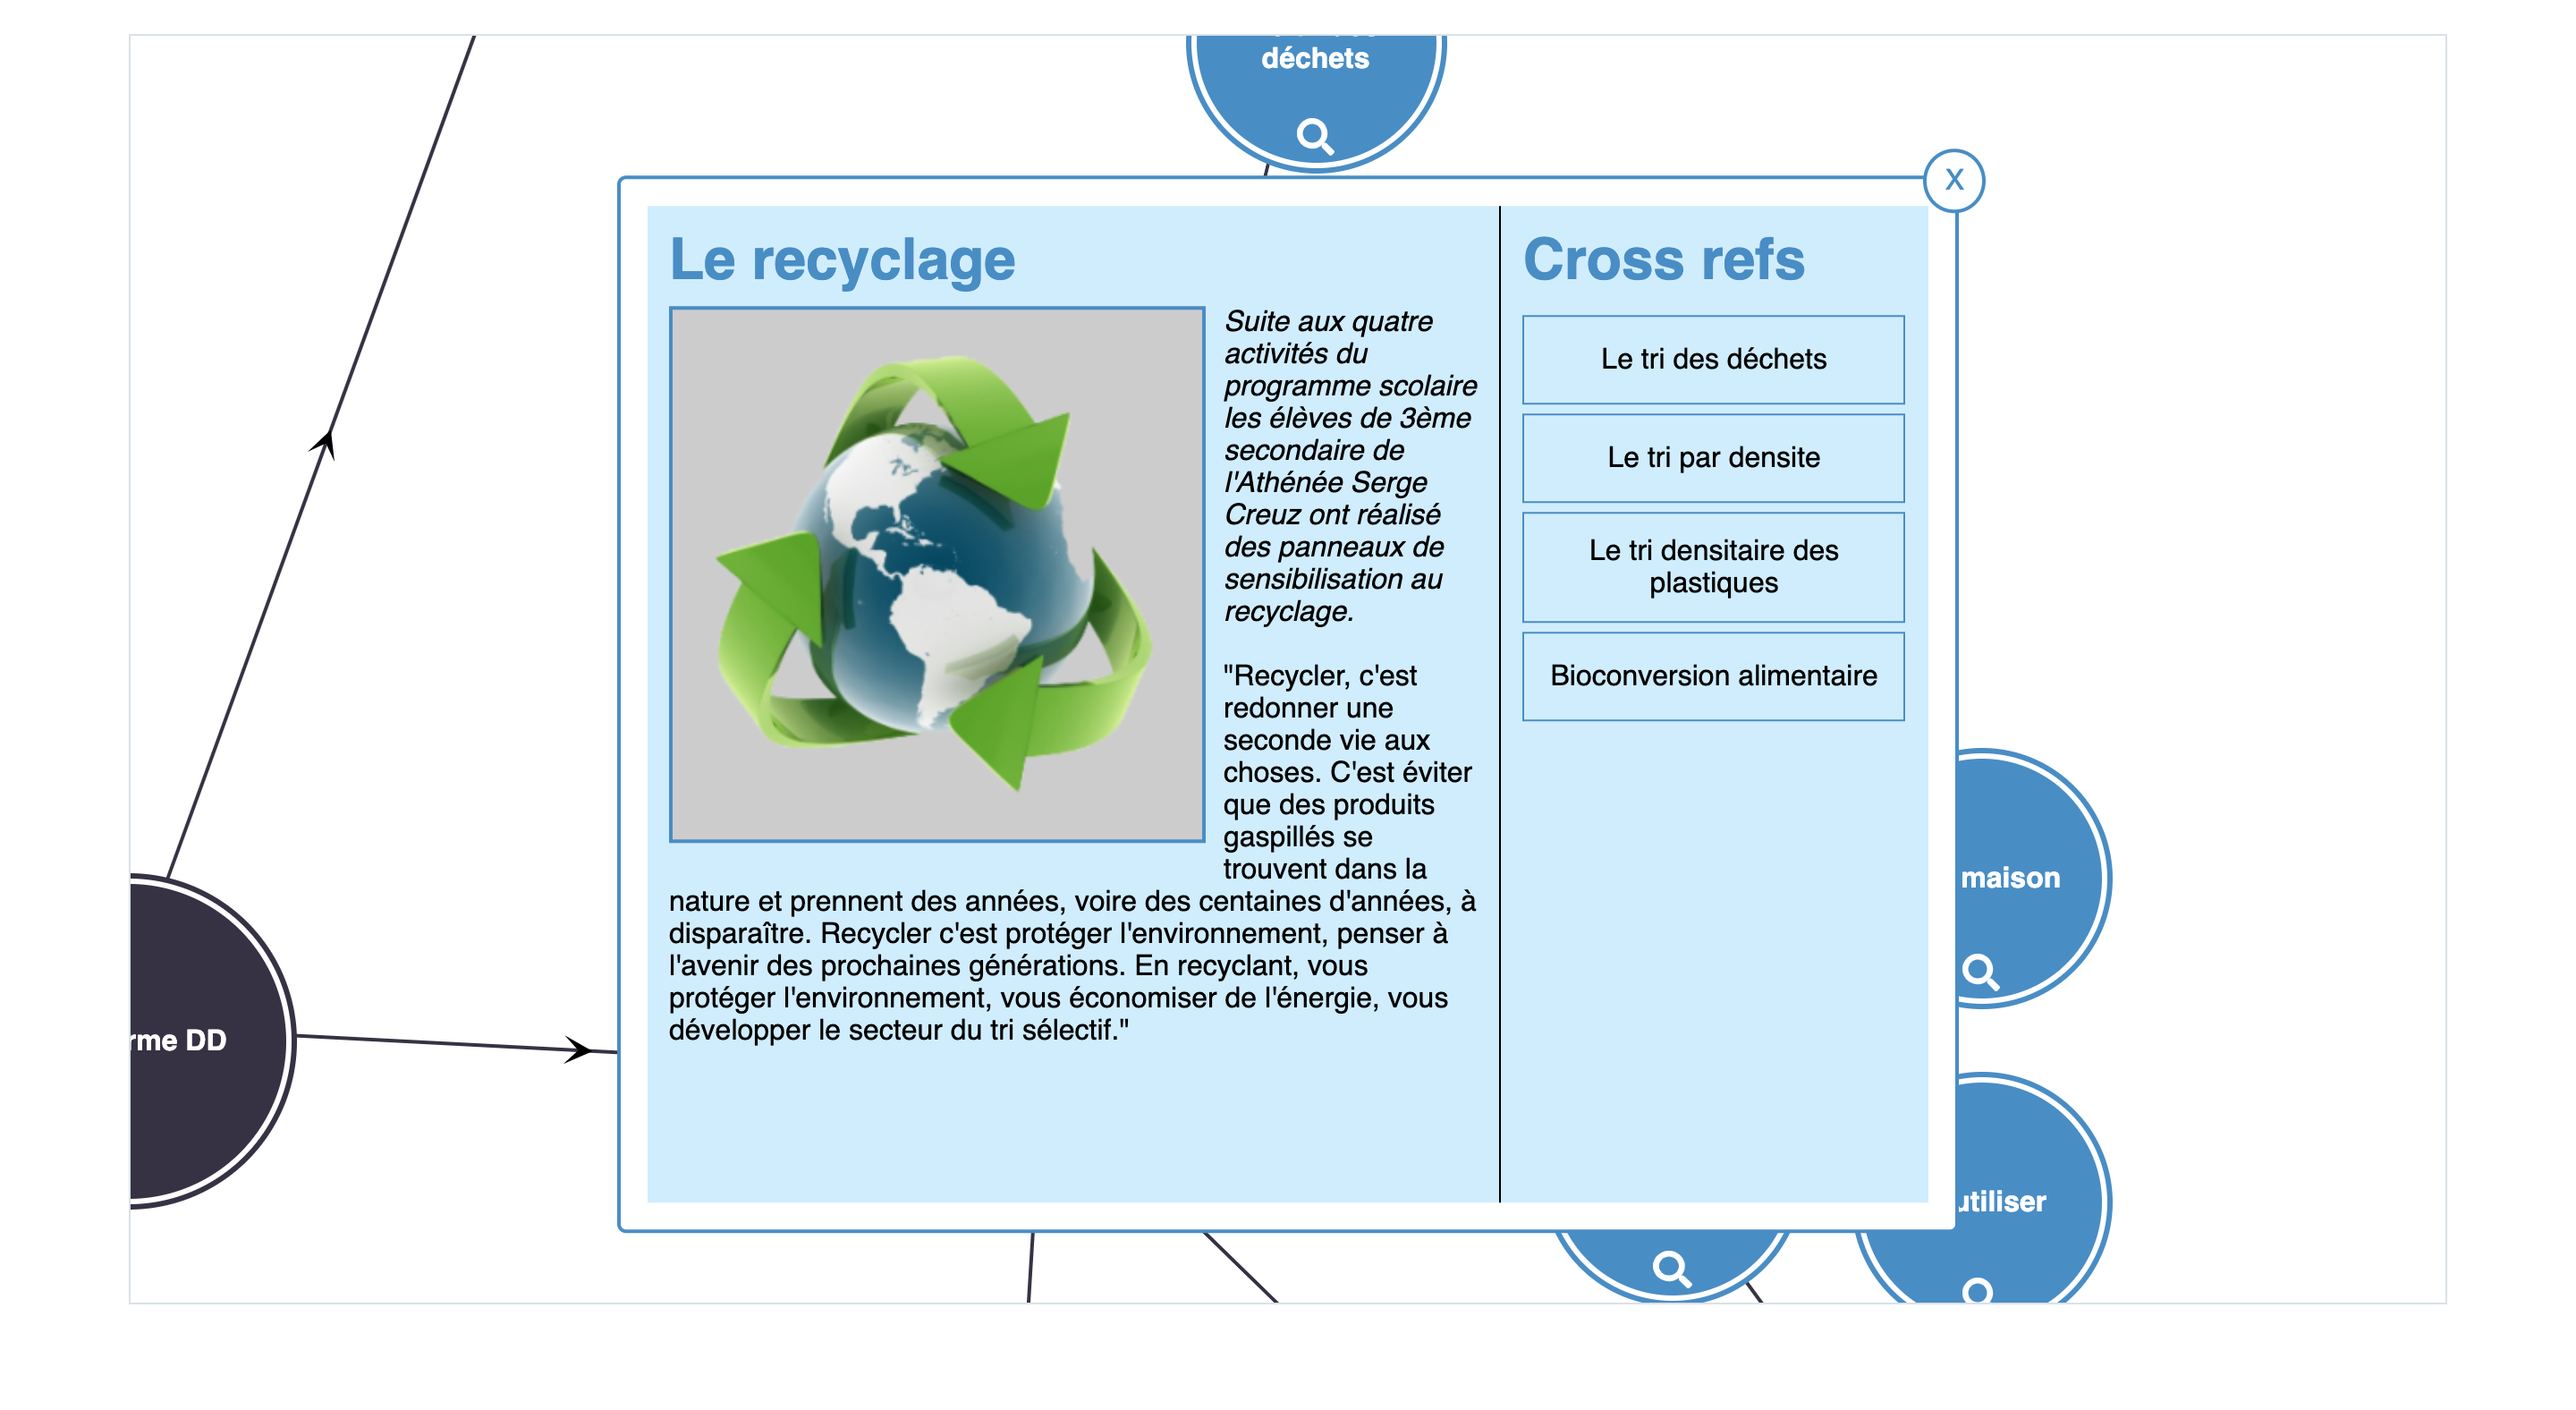
\includegraphics[width=\linewidth]{usecase/PDDEditModal.png}}
	\caption{Plateforme DD Edit Modal.}
	\label{fig:pdd-editmodal}
\end{figure}

At the left part of the modal, the actual content is shown. It starts with the title of the node, followed by a picture. If no picture exists, the text providing more information about the topic of the node is shown immediately under the title. Otherwise the title and the text are separated by the picture.\\

The size of the modal is fixed, but in case the information does not fit the modal, the user can scroll in the left part to continue reading until the end. The modal will never grow in size to make sure all data fits in it.\\

For some nodes, the modal will contain a list of so-called ``cross references'', which are links to nodes that in some way are related and which are not a direct child of the node. Such a link is not shown in the visualization, but by providing such a list, the user can still discover them. A click on a cross reference will close the modal and \textit{move} the visualization until the node of the corresponding cross reference is centered. This allows the user to navigate to linked nodes without the need to show a spaghetti of links in the visualization.



\subsection{Action Listeners}\label{sec:usecase-actionlisteners}
In GuideaMaps, we have a controls-div (section \ref{sec:controls}) containing a number of buttons to allow the user to perform some actions. In Plateforme DD, we chose for another approach. Because we have circular nodes instead of rectangular, it is less convenient to position multiple buttons next to each other at the bottom of the node. Further, we don't need a button to add child nodes because this is not allowed in Plateforme DD. Hence, we only have two buttons: one to expand and collapse the child nodes and one to open the edit modal.\\

The button to open the node is positioned in the center at the bottom of the node. A click on that button opens the modal and centers the node such that it is in the middle of the screen when the user closes the modal. Specific to this implementation is that there is a second way to open the modal. If the user clicks once on the node, it is centered. If he clicks once more on the node (not necessarily on the button), the modal will open and the content will be shown. This is because a click on a centered node results in the same action as a click on the button to open the node.\\

The second button is one to expand or collapse the child nodes. As already said, we cannot position it next to the other button at the bottom of the node. Therefore we position it at the top-left of the boundary of the node. There, a circle is visible with a minus inside if the children are visible. A click on the minus will collapse the node such that the children are not visible anymore and the minus will be replaced by a plus. When the user clicks on that plus again, the exact opposite action will happen: the node will be expanded (i.e. the children of the node will be visible again) and the plus will be replaced by a minus.\\

Note that a plus and minus can be used here as symbols to expand and collapse a node. This is possible because there can be no confusion with the action of adding a child node in Plateforme DD. If this would be possible, other symbols should be used to avoid such confusion and to not reduce the intuitiveness (requirement \ref{ur:icons}).



\clearpage

\chapter{Evaluation}\label{ch:evaluation}

In our tool, usability and user experience are very important. Therefore, we did two user studies. The first was to test the functionality of the GuideaMaps (as map creator and as end-user), while the second tested the use case about Plateforme DD.\\

This chapter is divided in two sections. The first describes the user study of GuideaMaps together with its results. In the second section, the same is done for the user study of Plateforme DD.





\section{GuideaMaps}

\subsection{Tasks \& Questions}

\subsection{Results}





\section{Plateforme DD}
The evaluation of the use case about Plateforme DD is different in comparison to the one about GuideaMaps. A first difference is that our audience is different: for GuideaMaps we chose for participants with a background in Computer Science to take the role as map creator. The participants taking the role of end-user were also more than 20 years old. Now, for Plateforme DD, our audience is between ten and fifteen years old. This is because the content on the website\footnote{\url{https://sciences.brussels/dd/}} was created by children of similar ages \textcolor{red}{(TODO: check this)}. However, the participants of the user study never worked with the website before.

\subsection{Setup}
The children were divided in two groups: one group solved the questionnaire using the website, while the other group solved the same questionnaire using the application. There was one tablet per two children on which the website or the application was running (depending on the group they were in). It was important they did not work with both systems because then there was the possibility a learning effect of having used one system before the other could influence the results. 

\subsection{Tasks \& Questions}
The user study consisted of different tasks and questions the children had to solve. Before they started with the actual tasks and questions, we gave them five to ten minutes to explore the website or the application so that they could get used to it a bit. We mentioned that it was important to understand the structure as much as possible because some questions would follow after this introduction period.\\

After five to ten minutes, we distributed the papers with the tasks and the questions. With other words, all children (of both groups) received part 1 of the questionnaire (see Appendix \ref{appendix:pdd-questionnaire}). \textcolor{red}{TODO: describe questions and tasks}\\



\subsection{Results}




\clearpage

\chapter{Conclusion \& Future Work}\label{ch:conclusion-future-work}

\section{Conclusion}\label{sec:conclusion}
In this thesis, we examined different visualization techniques in multiple domains. We started with a discussion of existing techniques and tools. It was clear that these were not very suitable for the goals we had in mind. We wanted a tool able to represent linked data and knowledge in a visual manner. Therefore, GuideaMaps was a good starting point. However, GuideaMaps had a number of limitations. First, the tool was created for iPads only. Hence, users were limited to a specific device and operating system. Further, there was no way to change the layout of the nodes and links. This thesis presented a solution to these and other limitations: GuideaMaps 2.0.\\

To achieve the goals (\autoref{sec:research-goals}) and requirements (\autoref{sec:requirements}), some crucial design decisions were made. The goal to have a device- and OS-independent application was achieved by the choice for a browser-based solution. In this way, users are not restricted to a particular device or OS anymore. Note that Google Chrome is currently the only browser in which the tool is tested, so other browsers can have a different (unexpected) behaviour.\\

Another difference with the first version of GuideaMaps is that we made it easier to create template maps. In the first version, this had to be done with XML, while we now have a graphical way to do this. This feature should make it easier for users with less background in Computer Science to create templates.\\

The biggest contribution of this thesis can be found in the genericity of our application. A tool that can be used for much more than only one domain (e.g. requirement elicitation) is a feature most people really like. Therefore, our application is created as a library. Developers can reuse the core of our application and replace the code responsible for the visualization of the nodes and links by their own implementation. The code can simply be plugged in without affecting the general implementation.\\

We strongly believe that this is a feature developers will like and tested the ease to plug in other code by means of a use case, i.e. Plateforme DD. It takes only a minute to plug in a custom implementation and run the library. The use case was also coupled to an evaluation of the visualization tool. Half of the participants worked with a website with a tree structure under the hood, while the other half worked with the same content of the website visualized by our application. The intent of visualizing the content was to make the structure more understandable. The results of the questionnaire confirmed our expectations: searching and finding information is easier when using our application than the website.


\section{Future Work}\label{sec:future-work}

The presented application could be improved in different ways in the future. One of the most important improvements that could be done is supporting a broader range of browsers. Currently, the tool works perfectly in the latest version of Google Chrome. It is good to have a working tool in one of the most widely used browsers, but lots of people use other browsers apart from Google Chrome. We detected some issues in Firefox, where for instance the tool is very slow on a tablet. In the future, we should improve the system such that it works in different browsers and if possible in all commonly used ones.\\

Furthermore, it is essential to be able to store the created templates and maps. Therefore, the system should be further elaborated so that the changes are written to a file that can be loaded the next time the map is opened. Right now, the maps are re-initialized every time the page is refreshed.\\

Next to supporting persistence, it would be useful to make the tool collaborative, i.e. allow multiple people to work simultaneously on the same map and see each others (saved) changes in real-time.\\

Another important improvement would be to make it possible to drag and drop the nodes of the visualization to support the similarity and proximity principle of the Gestalt Psychology Theory \citep{koffka2013principles}.\\

\clearpage

%\appendix
%renewcommand{\chaptermark}[1]{\markboth{\MakeUppercase{\appendixname}\ \thechapter.\ #1}{}}
%\chapter{Your Appendix} \label{App:AppendixA}
\addtocontents{toc}{\protect\setcounter{tocdepth}{0}}


\appendix
%\renewcommand{\bibname}{References\hfill}
\renewcommand{\bibsection}{\chapter{\refname}}
%\cleardoublepage
\bibliographystyle{apacite}
\bibliography{thesisbib} % change to your bib!
%\addcontentsline{toc}{section}{References}

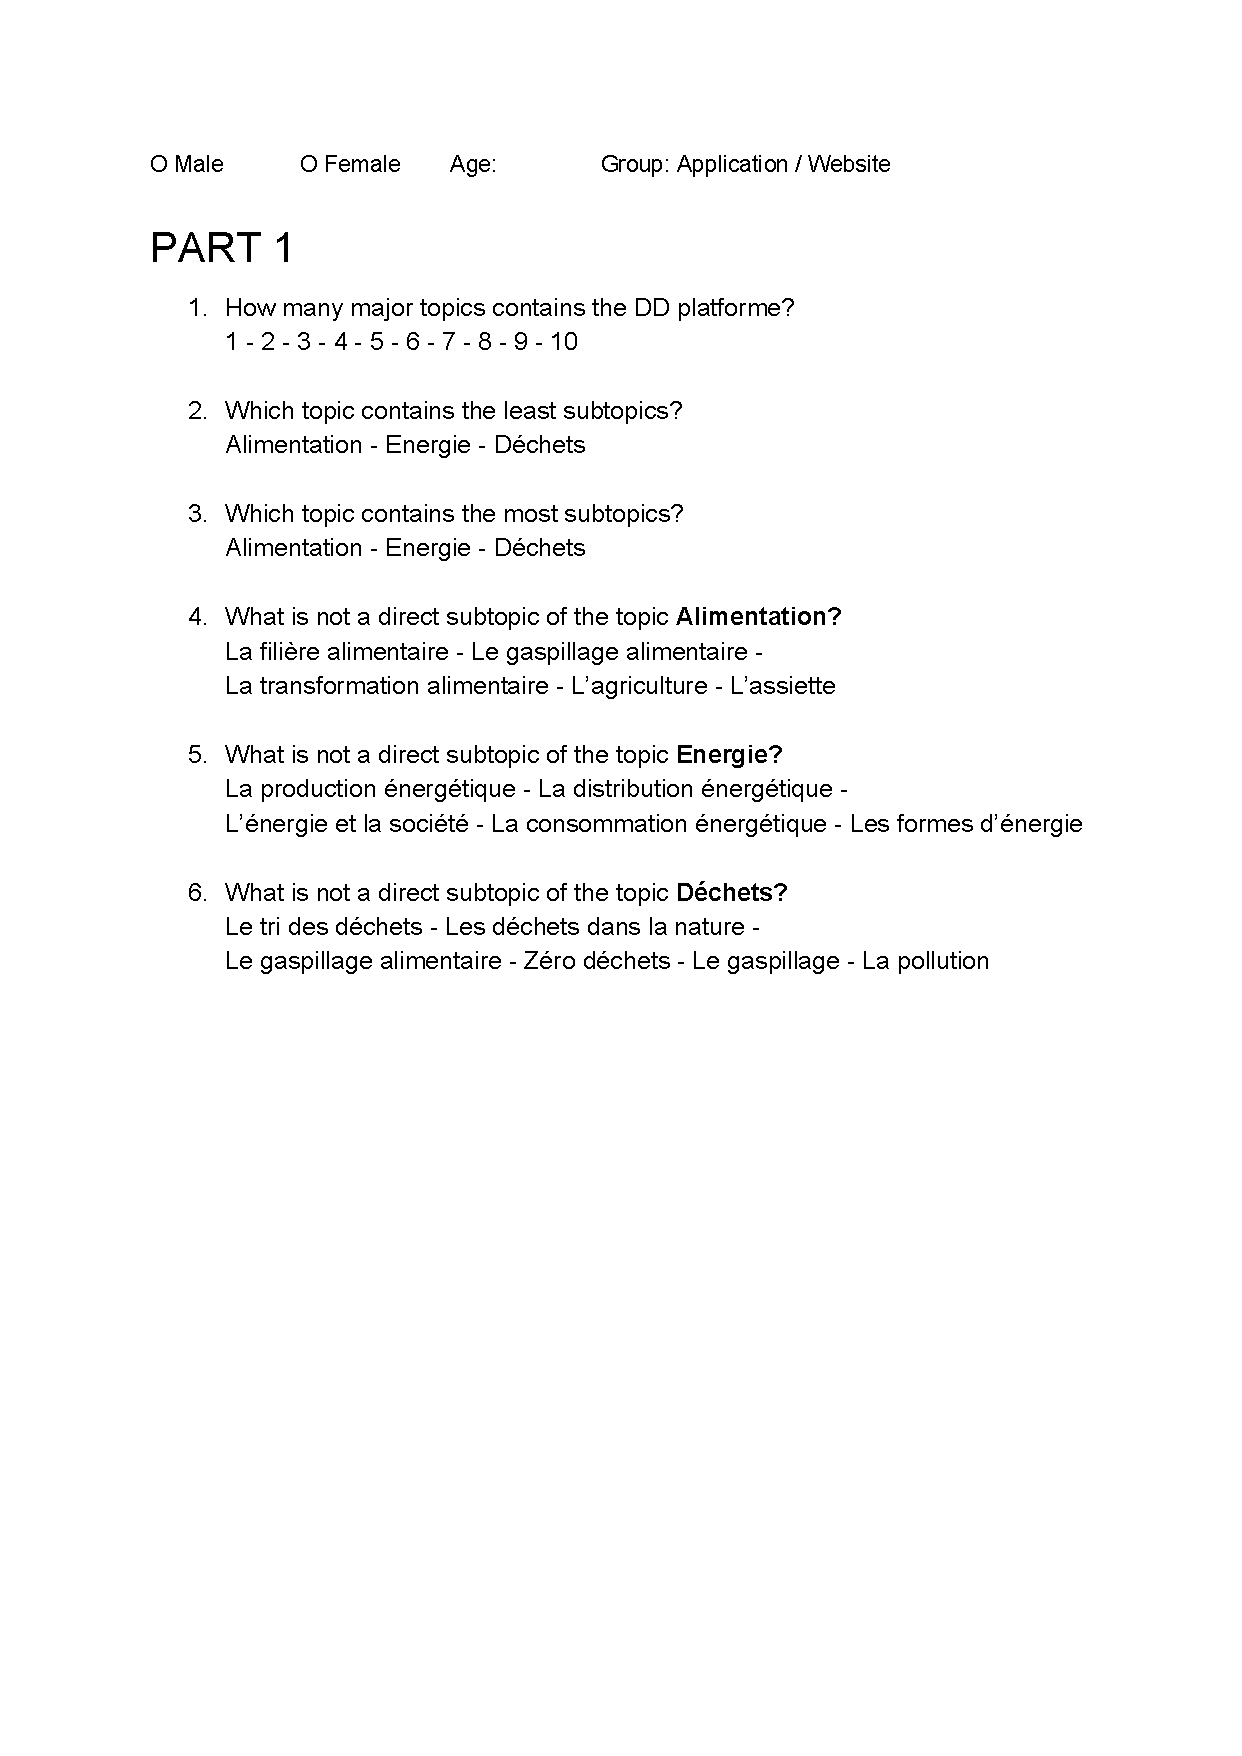
\includepdf[pages=1,pagecommand={\pagestyle{fancy}\chapter{Plateforme DD Questionnaire\label{appendix:pdd-questionnaire}}},offset=0 -10cm]{sections/PDDQuestionnaire.pdf}
\markboth{Plateforme DD Questionnaire}{Plateforme DD Questionnaire} % ensure the correct name appears in the header and footer
\includepdf[pages=2-,pagecommand={\pagestyle{fancy}}]{sections/PDDQuestionnaire.pdf}
\clearpage

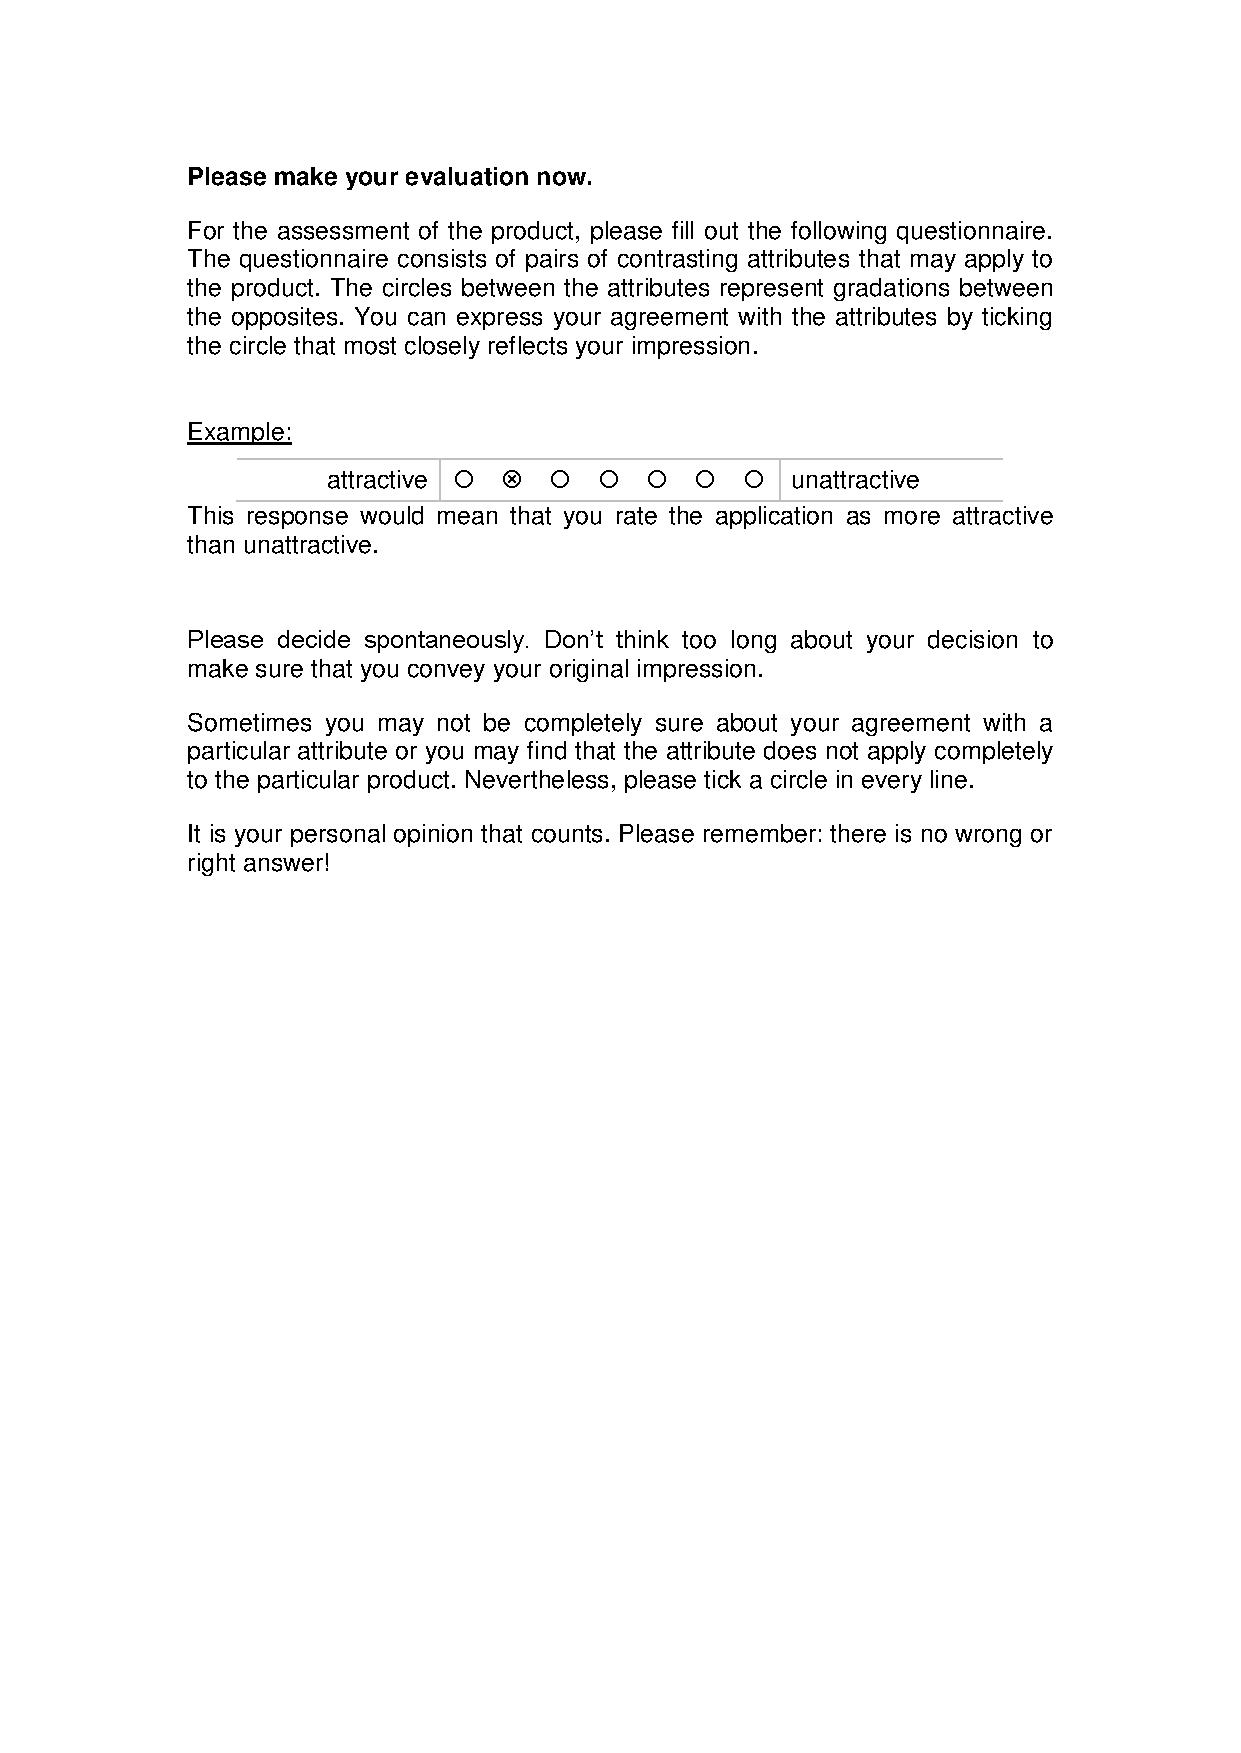
\includepdf[pages=1,pagecommand={\pagestyle{fancy}\chapter{User Experience Questionnaire\label{appendix:ueq-questionnaire}}},offset=0 -10cm]{sections/UEQ_English.pdf}
\markboth{User Experience Questionnaire}{User Experience Questionnaire} % ensure the correct name appears in the header and footer
\includepdf[pages=2-,pagecommand={\pagestyle{fancy}}]{sections/UEQ_English.pdf}
\clearpage


\end{document}
